\documentclass[10pt]{article}

\usepackage[utf8]{inputenc}
\usepackage{tabularx}
\usepackage{hyperref}
\usepackage{array}
\usepackage{graphicx}
\usepackage{geometry}
\usepackage{fancyhdr}
\usepackage{tikz}
\usepackage{ragged2e}
\usepackage{anyfontsize}
\usepackage[table,xcdraw]{xcolor}
\usepackage{tabularx, etoolbox}
\usepackage{eso-pic}
\usepackage{titlesec}
\usepackage{float}
\usepackage{longtable}

\newcommand\version{1.0.0} %aggiunta versione come variabile

\graphicspath{{images}}
%\graphicspath{{../images/}}

% Imposta il livello di profondità dell'indice
\setcounter{tocdepth}{4} % Aggiunge paragraph all'indice

% Abilita la numerazione fino a paragraph
\setcounter{secnumdepth}{5} % Estende la profondità della numerazione

% Ridefinizione dello stile di paragraph per includere la numerazione
\renewcommand\theparagraph{\thesubsubsection.\arabic{paragraph}}
\titleformat{\paragraph}
  {\normalfont\normalsize\bfseries}{\theparagraph}{1em}{}
\titlespacing*{\paragraph}
  {0pt}{1ex plus .2ex}{1ex plus .2ex}

% Ridefinizione dello stile di subparagraph per includere la numerazione
\renewcommand\thesubparagraph{\theparagraph.\arabic{subparagraph}}
\titleformat{\subparagraph}
  {\normalfont\normalsize\itshape}{\thesubparagraph}{1em}{}
\titlespacing*{\subparagraph}
  {0pt}{1ex plus .2ex}{1ex plus .2ex}

%cambio misure della pagina
\geometry{a4paper,left=25mm,right=25mm,top=25mm,bottom=25mm}
\definecolor{colorePie}{HTML}{ebdfc7}

% Header per ogni pagina
\pagestyle{fancy}
\fancyhf{}
\renewcommand{\headrulewidth}{0.4pt}
\lhead{
    \parbox[c]{1cm}{\includegraphics[width=1.1cm]{Sevenbitslogo.png}}
}
\rhead{\textcolor[HTML]{9e978a}{ NORME DI PROGETTO v\version}
}
\setlength{\headheight}{25pt}
\cfoot{\thepage}

% Indice
\renewcommand{\contentsname}{Indice}
\renewcommand{\listfigurename}{Elenco delle figure}
\renewcommand{\listtablename}{Elenco delle tabelle}

\begin{document}

% Pagina del titolo
\begin{titlepage}
    \setcounter{page}{0}
    \centering
    % Inserisci il logo del gruppo (modifica il percorso dell'immagine)
    \includegraphics[width=7.2cm]{Sevenbitslogo.png} \\[2cm]
    % Titolo
     {\fontsize{40}{40}\bfseries Norme di Progetto}\selectfont \\[3.9em]
    % Sottotitolo
        % Email del gruppo
    {\large sevenbits.swe.unipd@gmail.com} \\[3em]

    \hfill % Spazio per il logo dell'università
    \AddToShipoutPictureBG{ % Imposta il triangolo con logo
        \ifnum\value{page}=0
        \begin{tikzpicture}[overlay]
            % Definisce un triangolo blu in basso a destra
            \fill[colorePie]
                (current page.south east) -- ++(-9cm,0) -- ++(9cm,9cm);

            % Inserisce il logo all'interno del triangolo
            \node[anchor=south east, xshift=-0.3cm, yshift=0.3cm] at (current page.south east) {
                \includegraphics[width=4.5cm]{LogoUnipd.png}
            };
        \end{tikzpicture}
        \fi
    }
    \vfill % Aggiunge spazio verticale per centrare il contenuto
\end{titlepage}
\newpage
\clearpage
\setcounter{page}{1}

% Registro Modifiche
\begin{center}
\textbf{Registro modifiche}\\   
\end{center}

\renewcommand{\arraystretch}{1.5}
\rowcolors{0}{gray!11}{white} % Aggiunge colore alle righe del registro

\begin{longtable}{|>{\centering\arraybackslash}m{1.5cm}|>{\centering\arraybackslash}m{2cm}|>{\centering\arraybackslash}m{2.5cm}|>{\centering\arraybackslash}m{2.5cm}|>{\centering\arraybackslash}m{5cm}|}
\hline
\textbf{Versione} & \textbf{Data} & \textbf{Autore} & \textbf{Verificatore} & \textbf{Descrizione}\\
\endhead
    \hline
    1.0.0 & 2025-02-21 & Giovanni Cristellon & Manuel Gusella & Approvazione documento per RTB.\\
    \hline
    0.5.18 & 2025-02-17 & Federico Pivetta & Uncas Peruzzi & Correzioni ai nomi dei documenti\\
    \hline
    0.5.17 & 2025-02-17 & Leonardo Trolese & Federico Pivetta & Correzione minore di alcune \hyperref[metriche_qualita]{metriche}\\
    \hline
    0.5.16 & 2025-01-17 & Manuel Gusella & Uncas Peruzzi & Stesura metriche RSI$_G$ e CPI$_G$ nella sezione \hyperref[metriche_qualita]{Metriche per la qualità}\\
    \hline
    0.5.15 & 2025-01-16 & Manuel Gusella & Alfredo Rubino & Rimozione metriche non utilizzate e cambiamento dei codici delle metriche nella sezione \hyperref[metriche_qualita]{Metriche per la qualità}\\
    \hline
    0.5.14 & 2025-01-15 & Leonardo Trolese & Alfredo Rubino & Aggiunta delle metriche Fan IN e Fan OUT nella sezione delle \hyperref[metriche_qualita]{metriche}\\
    \hline
    0.5.13 & 2025-01-11 & Manuel Gusella & Leonardo Trolese & Aggiunte tabelle delle metriche per le sezioni \hyperref[codifica]{Codifica}, \hyperref[progettazione]{Progettazione} e \hyperref[analisi]{Analisi dei Requisiti}\\
    \hline
    0.5.12 & 2025-01-02 & Leonardo Trolese & Uncas Peruzzi & Aggiunta della metrica Function Point e correzioni minori\\
    \hline
    0.5.11 & 2025-01-02 & Leonardo Trolese & Uncas Peruzzi & Scrittura della sezione \hyperref[standard_12207]{"Standard ISO/IEC 12207"}\\
    \hline
    0.5.10 & 2024-12-27 & Leonardo Trolese & Uncas Peruzzi & Aggiunta immagine descrittiva nella sezione \hyperref[standard_9126]{"Standard ISO/IEC 9126"}\\
    \hline
    0.5.9 & 2024-12-27 & Federico Pivetta & Riccardo Piva & Completate sottosezioni \hyperref[miglioramento]{"Miglioramento"} e \hyperref[formazione]{"Formazione"}\\
    \hline
    0.5.8 & 2024-12-27 & Leonardo Trolese & Uncas Peruzzi & Aggiornamento della sezione \hyperref[standard_9126]{"Standard ISO/IEC 9126"}\\
    \hline
    0.5.7 & 2024-12-27 & Federico Pivetta & Uncas Peruzzi & Completata sottosezione \hyperref[gestione-configurazione]{"Gestione della configurazione"}\\
    \hline
    0.5.6 & 2024-12-26 & Alfredo Rubino & Riccardo Piva & Stesura della sottosezione "Gestione della qualità"\\
    \hline
    0.5.5 & 2024-12-24 & Riccardo Piva & Uncas Peruzzi & Ulteriore continuazione \hyperref[metriche_qualita]{stesura metriche}\\
    \hline
    0.5.4 & 2024-12-24 & Leonardo Trolese & Riccardo Piva & Continuazione stesura sezione metriche\\
    \hline
    0.5.3 & 2024-12-19 & Manuel Gusella & Alfredo Rubino & Fine stesura sottosezione \hyperref[verifica]{Verifica}\\
    \hline
    0.5.2 & 2024-12-18 & Manuel Gusella & Alfredo Rubino & Continuazione sottosezione \hyperref[verifica]{Verifica}\\
    \hline
    0.5.1 & 2024-12-16 & Manuel Gusella & Alfredo Rubino & Stesura iniziale della sottosezione \hyperref[verifica]{Verifica}\\
    \hline
    0.5.0 & 2024-12-16 & Alfredo Rubino & Manuel Gusella & Aggiunta sezione "Metriche per la qualità" e inizio stesura\\
    \hline
    0.4.3 & 2024-12-11 & Federico Pivetta & Manuel Gusella & Completata sottosezione "Gestione dei processi"\\
    \hline
    0.4.2 & 2024-12-11 & Leonardo Trolese & Manuel Gusella & Inizio scrittura sezione 5 relativa agli standard e correzione errori di battitura\\
    \hline
    0.4.1 & 2024-12-06 & Alfredo Rubino & Giovanni Cristellon & Aggiunte generali e correzioni\\
    \hline
    0.4.0 & 2024-12-06 & Federico Pivetta & Alfredo Rubino & Inizio stesura sottosezione "Gestione dei processi" e abbandono impostazione in sottodocumenti\\
    \hline
    0.3.9 & 2024-12-05 & Alfredo Rubino & Leonardo Trolese & Completata sezione "Processi Primari"\\
    \hline
    0.3.8 & 2024-12-05 & Federico Pivetta & Leonardo Trolese & Completato paragrafo "Diagrammi delle classi"\\
    \hline
    0.3.7 & 2024-12-04 & Alfredo Rubino & Leonardo Trolese & Aggiornamento sottosezione "Sviluppo" (terza parte) e completata modifica ai termini del Glossario\\
    \hline
    0.3.6 & 2024-12-04 & Federico Pivetta & Leonardo Trolese & Aggiornata sottosezione "Sviluppo" (seconda parte)\\
    \hline
    0.3.5 & 2024-12-02 & Alfredo Rubino & Giovanni Cristellon & Aggiornata sottosezione "Sviluppo"\\
    \hline
    0.3.4 & 2024-11-30 & Leonardo Trolese & Giovanni Cristellon & Correzioni grammaticali e di contenuti non più aderenti al Way-of-working$_G$ stabilito\\
    \hline
    0.3.3 & 2024-11-30 & Alfredo Rubino & Giovanni Cristellon & Aggiornata sottosezione "Sviluppo" e aggiunti livelli di profondità nell'indice\\
    \hline
    0.3.2 & 2024-11-28 & Alfredo Rubino & Giovanni Cristellon & Modifica ai termini del Glossario\\
    \hline
    0.3.1 & 2024-11-25 & Federico Pivetta & Riccardo Piva & Completata sottosezione "Fornitura" e aggiunta sottosezione "Sviluppo"\\
    \hline
    0.3.0 & 2024-11-24 & Federico Pivetta & Riccardo Piva & Aggiunta sezione "Processi primari"\\
    \hline
     0.2.1 & 2024-11-21 & Federico Pivetta  & Riccardo Piva & Completata sezione "Introduzione" e sottosezione "Documentazione", inclusa modifica alla tabella Registro modifiche\\
    \hline
    0.2.0 & 2024-11-20 & Leonardo Trolese & Federico Pivetta & Aggiunta sezione "Processi di supporto" e impostazione della divisione in sottodocumenti\\
    \hline
    0.1.0 & 2024-11-11 & Leonardo Trolese & Federico Pivetta & Creazione del documento secondo la struttura definita dal gruppo\\
    \hline
\end{longtable}
\rowcolors{0}{}{} % Riporta le righe alla colorazione originale

\newpage
\tableofcontents
\newpage
\listoffigures
\newpage
\listoftables

\newpage
\begin{justify}

\section{Introduzione}
    \subsection{Scopo del documento}
    Il presente documento è stato realizzato al fine di definire e raccogliere le best-practices$_G$ e il way-of-working$_G$ a cui ogni componente del gruppo Seven Bits dovrà aderire per l'intera realizzazione del progetto$_G$, garantendo così l'adozione di un metodo di lavoro completamente omogeneo.\\
    La formulazione delle norme$_G$ di progetto$_G$ avviene in maniera progressiva, permettendo al gruppo di apportare continui aggiornamenti ad esse in risposta alle esigenze che il team dovrà affrontare durante lo svolgimento del progetto$_G$ stesso.\\

    \subsection{Scopo del prodotto}
    Ogni giorno, le persone vengono sommerse da una miriade di annunci generici che spesso non rispecchiano i loro reali interessi o il contesto in cui si trovano. Questa separazione tra il messaggio e il destinatario porta ad una bassa interazione con gli utenti e una riduzione delle conversioni per i brand.\\
    Il progetto$_G$ “Near You” si concentra sulla creazione di una dashboard$_G$ composta principalmente da una mappa, sulla quale verranno visualizzate in tempo reale le posizioni degli utenti. Mediante un pop-up o una finestra a parte, verranno visualizzati messaggi personalizzati solo in prossimità dei punti di interesse.\\
    L'obiettivo finale è generare annunci pubblicitari in base agli interessi del cliente e alla sua posizione in quel momento.\\

    \subsection{Glossario}
    Ai fini di garantire l'adesione dei membri del gruppo ad un vocabolario comune e condiviso, che non lasci spazio ad ambiguità, dubbi o imprecisioni; il gruppo ha definito un documento denominato \textit{Glossario\_v1.0.0.pdf}, nel quale sono presenti tutti i termini tecnici adottati dal gruppo per l'intera durata della realizzazione del progetto$_G$. Tali termini saranno contrassegnati con una $_G$ a pedice. Nel caso di termini composti, essi saranno uniti da un trattino (es. pull-request$_G$)

    \subsection{Riferimenti}
        \subsubsection{Riferimenti normativi}
        \begin{itemize}
            \item Capitolato$_G$ di progetto$_G$ C4 - Near You - Smart custom advertising platform\\ \textcolor{blue}{\texttt{\url{https://www.math.unipd.it/~tullio/IS-1/2024/Progetto/C4p.pdf}}}\\ 
              (Consultato: 2025-02-19).
            \item Standard ISO/IEC 12207:1995\\ \textcolor{blue}{\texttt{\url{https://www.math.unipd.it/~tullio/IS-1/2009/Approfondimenti/ISO_12207-1995.pdf}}}\\
              (Consultato: 2025-02-19).
        \end{itemize}
        \subsubsection{Riferimenti tecnologici}
        \begin{itemize}
            \item Documentazione$_G$ Git$_G$: \textcolor{blue}{\texttt{\url{https://git-scm.com/docs}}}\\
              (Consultato: 2025-02-19).
            \item Documentazione$_G$ Github$_G$: \textcolor{blue}{\texttt{\url{https://docs.github.com/en}}}\\
              (Consultato: 2025-02-19).
            \item Documentazione$_G$ \LaTeX: \textcolor{blue}{\texttt{\url{https://www.latex-project.org/help/documentation/}}}\\
              (Consultato: 2025-02-19).
            \item Documentazione$_G$ Python$_G$: \textcolor{blue}{\texttt{\url{https://www.python.org/doc/}}}\\
              (Consultato: 2025-02-19).
        \end{itemize}
        \subsubsection{Riferimenti informativi}
        \begin{itemize}
            \item Riferimenti per le metriche: 
            \begin{itemize}
                \item \textcolor{blue}{\texttt{\url{https://www.javatpoint.com/software-engineering-functional-point-fp-analysis}}}\\
              (Consultato: 2025-02-19).\\
                \item \textcolor{blue}{\texttt{\url{https://lia.disi.unibo.it/Courses/IngSW/SE_C_2_Metriche_.pdf}}}\\
              (Consultato: 2025-02-19).\\
                \item \textcolor{blue}{\texttt{\url{https://www.valeriofinazzo.it/wordpress/2014/06/function-point-tutorial-2-definizioni/}}}\\
              (Consultato: 2025-02-19).\\
                \item \textcolor{blue}{\texttt{\url{https://youtu.be/CXgDazM0DWA?feature=shared}}}\\
              (Consultato: 2025-02-19).
            \end{itemize}
        \end{itemize}

\newpage
\section{Processi primari}
    \subsection{Fornitura}

    \subsubsection{Descrizione e Scopo}
    Come stabilito dallo standard ISO/IEC 12207:1995, il processo$_G$ di fornitura definisce un insieme di linee guida necessario per una buona comunicazione tra fornitore e proponente$_G$. Il processo$_G$ di fornitura si occupa di controllare e coordinare tutte le attività svolte dal gruppo, dalla comprensione dei requisiti fino alla consegna, per garantire che il prodotto finale soddisfi le esigenze concordate con la proponente$_G$.\\

    \subsubsection{Attività}
    Il processo$_G$ di fornitura, come stabilito dallo standard ISO/IEC 12207:1995, si compone delle seguenti attività:
    \begin{enumerate}
        \item \textbf{Avvio}: Composto dall'identificazione e comprensione delle richieste della proponente$_G$, con successiva verifica della fattibilità tecnologica di queste ultime;
        \item \textbf{Preparazione dell'offerta}: Composta dall'elaborazione della proposta in grado di soddisfare le richieste della proponente$_G$, che dettagli i requisiti, i tempi, i costi e le condizioni contrattuali;
        \item \textbf{Contrattazione}: Composta dalla collaborazione tra fornitore e proponente$_G$ per finalizzare i punti cardine della proposta;
        \item \textbf{Pianificazione}: Composta dalla pianificazione delle attività necessarie per soddisfare i requisiti della proponente$_G$, seguita da una suddivisione delle ore produttive disponibili ed una stima dei costi;
        \item \textbf{Esecuzione}: Composta dalla pianificazione e dallo sviluppo del prodotto in conformità ai requisiti concordati, insieme ad un monitoraggio continuo delle attività;
        \item \textbf{Revisione}: Composta dalla verifica periodica del progresso rispetto ai criteri definiti dal contratto;
        \item \textbf{Consegna}: Composta dalla consegna del prodotto software alla proponente$_G$, accompagnato dalla documentazione$_G$ finale.
    \end{enumerate}

    \subsubsection{Rapporti con l'azienda proponente$_G$}
    L'azienda proponente$_G$ SyncLab$_G$ si è resa disponibile mediante diversi canali tra cui: e-mail, Discord e Google Meet ad una comunicazione frequente con il gruppo Seven Bits, così da risolvere tempestivamente eventuali domande o dubbi che possono emergere durante lo svolgimento del progetto$_G$.\\
    Durante la prima riunione organizzativa con l'azienda, è stata definita l'organizzazione dei periodi di sprint$_G$, stabilendo una durata di due settimane per ciascun ciclo. Al termine di ogni sprint$_G$ avviene un incontro SAL$_G$ (Stato di Avanzamento Lavori), dove verranno analizzati i risultati del lavoro svolto e si procederà con una sprint-review$_G$. Inoltre, tra un SAL$_G$ e l'altro, secondo le necessità di proponente$_G$ e team, è possibile concordare un incontro intermedio per monitorare i progressi raggiunti e rispondere ad eventuali quesiti emersi.\\
    Ogni incontro con l'azienda viene formalizzato attraverso un verbale esterno. Tale verbale è successivamente sottoposto alla proponente$_G$ per la validazione mediante firma, in modo da ottenere un'approvazione formale del resoconto delle discussioni svolte durante la riunione.\\

    \subsubsection{Documentazione fornita}
    Di seguito sono elencati i documenti che il gruppo si impegna a consegnare ai Committenti, Prof. Tullio Vardanega e Prof. Riccardo Cardin, nonché all'azienda proponente$_G$:\\

        \paragraph{Analisi dei Requisiti}
        \'E un documento essenziale per lo sviluppo del prodotto software, che include la descrizione degli attori coinvolti, dei casi d'uso e l'elenco dei requisiti, suddivisi in requisiti funzionali, di qualità, di vincolo e prestazionali.\\

        \paragraph{Piano di Progetto$_G$}
        Il \textit{Piano\_di\_Progetto} è un documento che ha lo scopo di definire in modo chiaro le modalità con cui ogni membro del gruppo svolgerà le attività per la realizzazione del progetto$_G$. Include l'analisi dei rischi, la pianificazione delle attività, la suddivisione dei ruoli e la stima di costi e risorse.\\

        \paragraph{Piano di Qualifica}
        Il \textit{Piano\_di\_Qualifica} è un documento che ha l'obiettivo di garantire la qualità del prodotto e dei processi durante l'intero ciclo-di-vita$_G$ del progetto$_G$, per questo motivo sarà aggiornato nel tempo per riflettere eventuali modifiche e i risultati delle verifiche effettuate. Include le sezioni sulla qualità di processo$_G$, sulla qualità di prodotto, le modalità di testing e il cruscotto$_G$ di valutazione delle qualità.\\

        \paragraph{Glossario}
        Il \textit{Glossario} è un documento che raccoglie dei termini specifici e le loro definizioni chiare e concise. Il suo scopo è quello di facilitare la comprensione dei concetti chiave presenti nei vari documenti redatti.\\

        \paragraph{Lettera di Presentazione}
        La Lettera di Presentazione è un documento che accompagna la consegna del prodotto software e della relativa documentazione$_G$ durante le fasi di revisione di progetto$_G$. Il contenuto di questo documento comprende un link alla pagina web che contiene tutta la documentazione$_G$ fin'ora prodotta ed un preventivo aggiornato rispetto a quello presentato alla revisione precedente.\\

    \subsubsection{Strumenti}
    Gli strumenti utilizzati per la gestione del processo$_G$ di fornitura sono i seguenti:
    \begin{itemize}
        \item \textbf{Canva}: Piattaforma che permette la creazione di presentazioni multimediali, utilizzata per la realizzazione dei diari di bordo;
        \item \textbf{Draw.io}: Software utilizzato per creare diagrammi e grafici di vario tipo, in particolare è stato impiegato per realizzare diagrammi UML$_G$, come quelli dei casi d'uso;
        \item \textbf{Google Meet e Discord}: Servizi che permettono di effettuare videochiamate, utilizzati dal team per le discussioni sincrone e asincrone con la proponente$_G$;
        \item \textbf{Google Sheets}: Servizio che permette la creazione di fogli di calcolo, utilizzato dal gruppo per la rendicontazione delle ore produttive impiegate durante ogni sprint$_G$.
    \end{itemize}

    \subsection{Sviluppo}

    \subsubsection{Descrizione e Scopo}
    Il processo$_G$ di sviluppo rappresenta l'insieme delle attività necessarie per realizzare il prodotto software, garantendo il rispetto dei requisiti e delle scadenze concordate con la proponente$_G$. Questo processo$_G$ si articola in diverse fasi fondamentali, quali l'analisi-dei-requisiti, la progettazione, la codifica, l'integrazione, e la verifica, assicurando che ogni fase contribuisca al raggiungimento degli obiettivi prefissati.\\
    Le linee guida descritte in questa sezione sono volte a strutturare il lavoro in modo chiaro e uniforme, promuovendo la qualità del prodotto finale. Seguendo standard solidi e definiti, nel caso specifico l'ISO/IEC 12207:1995, si crea un ambiente di lavoro orientato a garantire la coerenza nei metodi utilizzati e il rispetto delle aspettative.\\
    L'obiettivo è consegnare un prodotto software di alta qualità, che soddisfi le esigenze richieste, rispettando le tempistiche e garantendo il successo del progetto$_G$.\\

    \subsubsection{Analisi-dei-Requisiti}
    \label{analisi}
        \paragraph{Descrizione e Scopo}
        L'Analisi-dei-Requisiti$_G$ è la prima fase cruciale del processo$_G$ di sviluppo software. Lo scopo principale di questa fase è definire con chiarezza le funzionalità e le caratteristiche che il sistema$_G$ dovrà offrire, in base alle necessità degli utenti. Per raggiungere tale obiettivo, è essenziale stabilire una comunicazione efficace con la proponente$_G$, assicurandosi che tutte le esigenze siano documentate e validate. Questo processo$_G$ permette di chiarire gli obiettivi del prodotto, identificare i vincoli operativi e fornire ai Progettisti le informazioni necessarie per sviluppare un'architettura coerente e un design adeguato. Il risultato di questa attività è formalizzato nel documento \textit{Analisi\_dei\_Requisiti}, redatto dagli Analisti, che contiene una descrizione dettagliata degli obiettivi del prodotto, delle funzionalità previste e delle caratteristiche degli utenti. Include inoltre una sezione dedicata ai casi d'uso, che descrivono le interazioni tra gli attori e il sistema$_G$.\\
        Infine, l'Analisi-dei-Requisiti$_G$ contribuisce a migliorare la comunicazione tra tutti gli stakeholder$_G$, agevola la pianificazione del progetto$_G$ in termini di tempistiche e costi e fornisce un riferimento chiaro per le attività di verifica e test$_G$.\\

        \paragraph{Casi d'uso}
        I casi d'uso rappresentano scenari concreti che descrivono come gli utenti e altri attori interagiranno con il sistema$_G$ per raggiungere obiettivi specifici. Questi scenari aiutano a identificare requisiti chiave e prevenire malintesi.\\
        È importante sottolineare che i diagrammi dei casi d'uso non si concentrano sui dettagli implementativi. Il loro scopo è quello di rappresentare le funzionalità del sistema$_G$ esclusivamente dal punto di vista esterno, evidenziando come esso interagisce con gli attori e soddisfa le loro esigenze.\\
        Ogni caso-d'uso$_G$ ha le seguenti caratteristiche:
        \begin{itemize}
            \item \textbf{Identificativo}:
            \begin{quote}
                \textbf{UC [Numero caso-d'uso$_G$] . [Numero sottocaso d'uso] - [Titolo]}
            \end{quote}
            Dove:
            \begin{itemize}
                \item \textbf{Numero caso-d'uso$_G$}: ID relativo al caso-d'uso$_G$ principale;
                \item \textbf{Numero sottocaso d'uso}: ID relativo allo specifico sottocaso d'uso (se applicabile);
                \item \textbf{Titolo}: Descrizione breve ed esplicativa;
            \end{itemize}

            \item \textbf{Attore principale}: Entità esterna che interagisce attivamente con il sistema$_G$ per raggiungere uno scopo, ad esempio un utente specifico o un altro sistema$_G$ esterno;
            \item \textbf{Attore secondario}: Eventuale entità esterna invocata dal sistema$_G$ per fornire un supporto, in modo da soddisfare il bisogno dell'attore principale;
            %\item \textbf{Descrizione}: Breve descrizione della funzionalità del caso-d'uso$_G$;
            \item \textbf{Scenario principale}: Sequenza di eventi che si susseguono da quando un attore$_G$ inizia ad interagire con il sistema$_G$;
            \item \textbf{Precondizioni}: Descrizione dello stato del sistema$_G$ necessario per attivare il caso-d'uso$_G$;
            \item \textbf{Postcondizioni}: Descrizione dello stato del sistema$_G$ al completamento del caso-d'uso$_G$;
            \item \textbf{Estensioni}: Eventuali scenari alternativi, descritti in questa sezione se presenti;
            \item \textbf{User story associata}: Funzionalità descritta dal punto di vista dell'utente, scritta in linguaggio naturale perché risulti semplice e comprensibile. Definita nella forma seguente: \newline
            \vspace{-5mm}
            \begin{center}
                - Come [utente], desidero poter [funzionalità] per [valore aggiunto]. -
            \end{center} 
        \end{itemize}

        \paragraph{Diagrammi dei casi d'uso}
        I diagrammi dei casi d'uso sono strumenti visivi che rappresentano le funzionalità del sistema$_G$ dal punto di vista dell'utente. Mostrano come gli attori esterni (utenti, dispositivi, altri sistemi) interagiscono con il sistema$_G$, senza entrare nei dettagli tecnici. Il loro obiettivo principale è descrivere le interazioni tra attori e sistema$_G$, facilitando la comprensione dei requisiti funzionali e la comunicazione tra gli stakeholder$_G$.\\
        Ogni caso-d'uso$_G$ descrive una sequenza di azioni che un attore$_G$ compie per raggiungere un obiettivo specifico. Questi casi sono interconnessi e rappresentano i flussi di lavoro principali, evidenziando come l'attore interagisce con il sistema$_G$. I diagrammi non trattano i dettagli implementativi, ma si concentrano sulle funzionalità, trattando il sistema$_G$ come un "black box" esterno.\\
        Di seguito sono elencati i principali componenti di un diagramma dei casi d'uso:
        \begin{itemize}
            \item \textbf{Attori}\\
            Gli attori sono entità esterne al sistema$_G$ che interagiscono con esso per utilizzare le sue funzionalità. Possono essere utenti umani, altri sistemi software, dispositivi, macchine o organizzazioni. Un caso-d'uso$_G$ definisce una specifica funzionalità che il sistema$_G$ fornisce agli attori, senza entrare nei dettagli implementativi. Nel diagramma dei casi d'uso, gli attori sono rappresentati da figure stilizzate posizionate all'esterno del rettangolo che delinea il sistema$_G$, e ciascuno è identificato da un'etichetta con il suo nome.
            \begin{figure}[H]
            \centering
            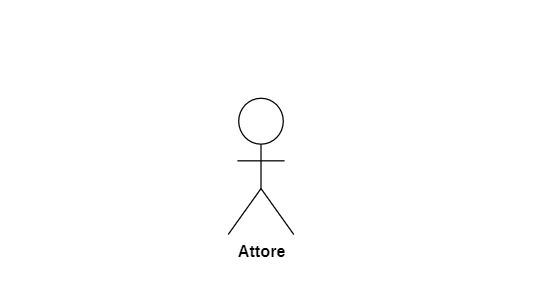
\includegraphics[width=0.45\textwidth]{Attore.PNG}
            \caption{Rappresentazione di un attore$_G$.}
            \end{figure}

            \item \textbf{Casi d'uso}\\
            Ogni caso-d'uso$_G$ identifica una specifica azione o funzionalità offerta dal sistema$_G$, con cui l'attore può interagire. I casi d'uso sono collegati tramite una linea continua agli attori che hanno accesso a quella funzionalità, creando una chiara relazione tra gli utenti e le azioni che possono compiere.\\
            Nel diagramma dei casi d'uso, ogni caso è rappresentato da una forma ovale contenente un ID univoco e un titolo esplicativo.
            \begin{figure}[H]
            \centering
            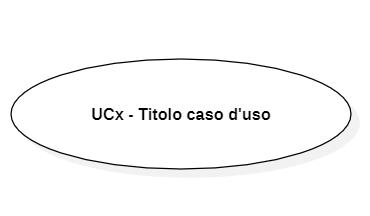
\includegraphics[width=0.30\textwidth]{UC.PNG}
            \caption{Rappresentazione di un caso-d'uso$_G$.}
            \end{figure}

            \item \textbf{Sottocasi d'uso}\\
            Un sottocaso d'uso rappresenta una versione più dettagliata di un caso-d'uso$_G$  generico. Esso offre un livello di dettaglio più approfondito sulle funzionalità o sui particolari scenari di utilizzo rispetto al caso-d'uso$_G$ principale. Non è obbligatorio per un caso-d'uso$_G$ possedere uno o più sottocasi.
            \begin{figure}[H]
            \centering
            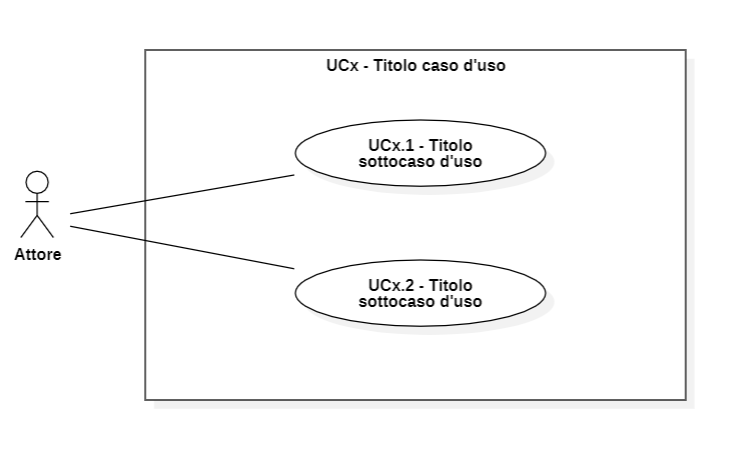
\includegraphics[width=0.6\textwidth]{SottoUC.PNG}
            \caption{Rappresentazione di un sottocaso d'uso.}
            \end{figure}

            \item \textbf{Sistema}\\
            Il sistema$_G$ viene rappresentato con un rettangolo all'interno del quale vengono collocati i casi d'uso. All'esterno del rettangolo sono invece posizionati i vari attori.
            \begin{figure}[H]
            \centering
            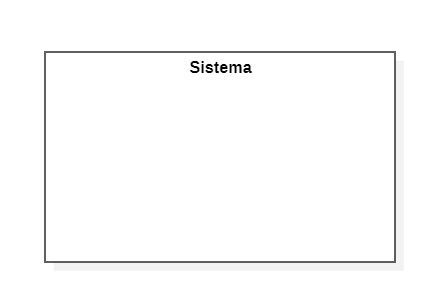
\includegraphics[width=0.4\textwidth]{Sistema.PNG}
            \caption{Rappresentazione di un sistema$_G$.}
            \end{figure}

            \item \textbf{Associazione}\\
            Una linea di associazione stabilisce una connessione tra un attore$_G$ e un caso-d'uso$_G$ quando l'attore è coinvolto nell'attività descritta dal caso-d'uso$_G$. Questo collegamento visivo rappresenta il ruolo dell'attore nell'attivare o nell'utilizzare una specifica funzionalità del sistema$_G$.
            \begin{figure}[H]
            \centering
            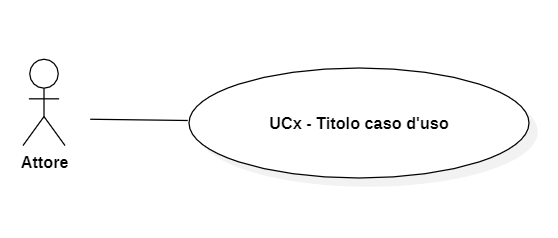
\includegraphics[width=0.5\textwidth]{AssociazioneAttore.PNG}
            \caption{Rappresentazione di una associazione tra attore$_G$ e UC.}
            \end{figure}

            \item \textbf{Generalizzazione (attori)}\\
            La generalizzazione tra attori rappresenta una relazione gerarchica in cui un attore$_G$ specializzato (figlio) eredita comportamenti e caratteristiche da un attore$_G$ base (genitore). Questo meccanismo aiuta a organizzare gerarchicamente gli attori nei diagrammi dei casi d'uso, definendo i casi d'uso che un attore$_G$ può utilizzare e che sono anche disponibili per gli attori più specializzati. La generalizzazione viene rappresentata con una linea solida e una freccia vuota che va dall'attore figlio all'attore genitore, indicando la direzione dell'eredità.
            \begin{figure}[H]
            \centering
            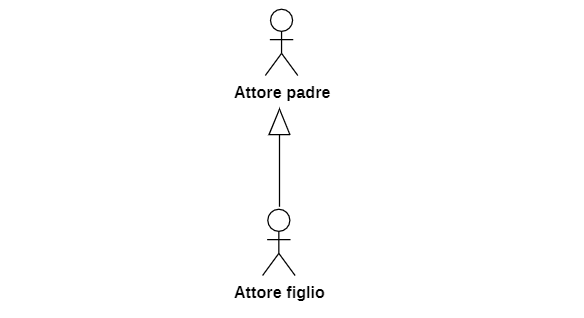
\includegraphics[width=0.5\textwidth]{GeneralizzazioneAttore.PNG}
            \caption{Rappresentazione di una generalizzazione tra attori.}
            \end{figure}

            \item \textbf{Inclusione}\\
            La relazione di inclusione indica quando un caso-d'uso$_G$ (includente) comprende l'esecuzione di un altro caso-d'uso$_G$ (incluso). Quando un attore$_G$ interagisce con il caso-d'uso$_G$ includente, il caso-d'uso$_G$ incluso viene eseguito automaticamente come parte di quest'ultimo. Questa relazione è utile per il riutilizzo delle funzionalità e per evitare la duplicazione delle stesse logiche in più casi d'uso. La relazione di inclusione viene rappresentata da una freccia tratteggiata che collega il caso-d'uso$_G$ incluso al caso-d'uso$_G$ includente.
            \begin{figure}[H]
            \centering
            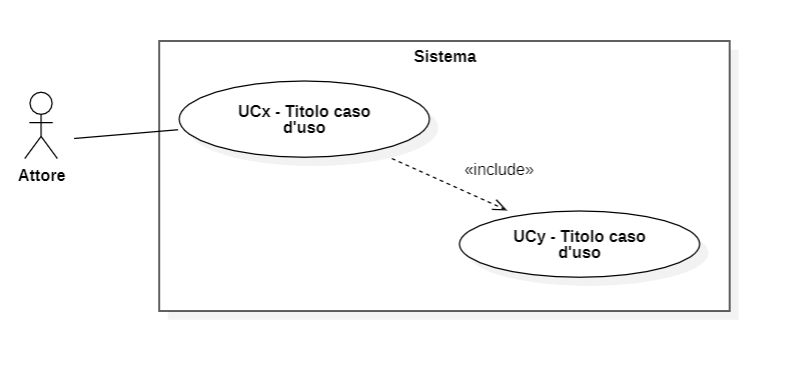
\includegraphics[width=0.6\textwidth]{InclusioneUC.PNG}
            \caption{Rappresentazione di una inclusione tra UC.}
            \end{figure}

            \item \textbf{Estensione}\\
            La relazione di estensione indica quando un caso-d'uso$_G$ (estendente) può modificare o arricchire il comportamento di un altro caso-d'uso$_G$ (esteso) in determinate circostanze. Questa relazione viene utilizzata quando un evento o una condizione porta il flusso del caso-d'uso$_G$ a deviare dallo scenario principale verso uno scenario alternativo, come nei casi di errore, ma mantenendo le stesse precondizioni del caso-d'uso$_G$ principale. La relazione di estensione è rappresentata da una freccia tratteggiata che collega il caso-d'uso$_G$ estendente al caso-d'uso$_G$ esteso.
            \begin{figure}[H]
            \centering
            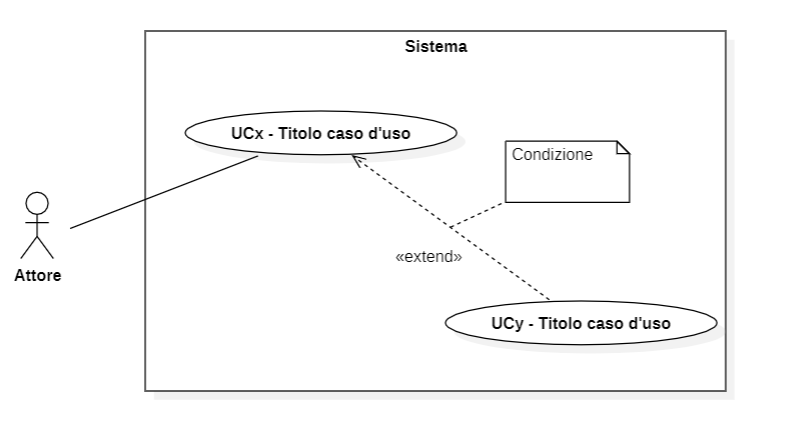
\includegraphics[width=0.6\textwidth]{EstensioneUC.PNG}
            \caption{Rappresentazione di una estensione tra UC.}
            \end{figure}

            \item \textbf{Generalizzazione (casi d'uso)}\\
            La generalizzazione nei diagrammi dei casi d'uso rappresenta una relazione di ereditarietà tra casi d'uso, in cui un caso-d'uso$_G$ più specifico eredita il comportamento da un caso-d'uso$_G$ più generico. Questa relazione è utile per definire funzionalità più dettagliate, ed è simboleggiata da una linea con una freccia vuota che va dal caso-d'uso$_G$ specifico al caso-d'uso$_G$ generico.
            \begin{figure}[H]
            \centering
            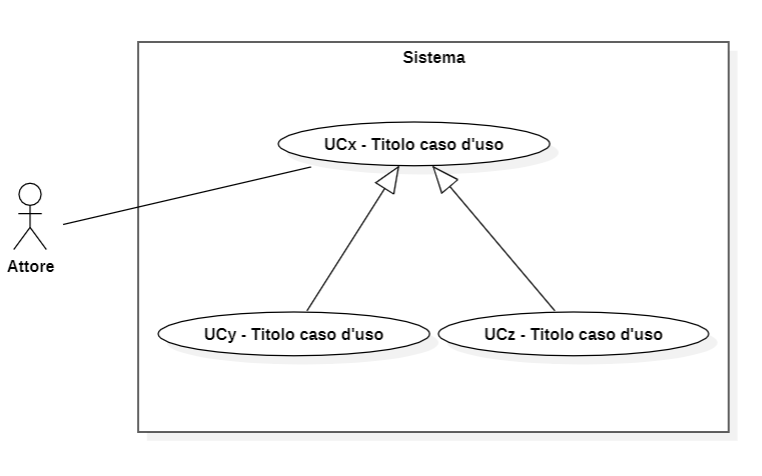
\includegraphics[width=0.55\textwidth]{GeneralizzazioneUC.PNG}
            \caption{Rappresentazione di una generalizzazione tra UC.}
            \end{figure}
        \end{itemize}

        \paragraph{Requisiti}
        I requisiti di un prodotto software sono specifiche documentate che delineano le funzionalità che il sistema$_G$ deve soddisfare. Essi fungono da guida per lo sviluppo, il testing e la validazione del prodotto, garantendo che risponda alle esigenze degli utenti e agli obiettivi del progetto$_G$. Ogni requisito$_G$ deve essere definito con precisione, e riflettere pienamente le attese del cliente o del proponente$_G$.\\
        Ad ogni requisito$_G$ è assegnato un grado di importanza:
        \begin{itemize}
            \item \textbf{Obbligatorio}: Essenziale per soddisfare le esigenze del proponente$_G$;
            \item \textbf{Desiderabile}: Utile ma non prioritario, può essere implementato in seguito;
            \item \textbf{Opzionale}: Aggiunge valore al prodotto, ma può essere tralasciato per motivi di costo o tempistica.
        \end{itemize}
        I requisiti si suddividono inoltre in tre diverse tipologie:
        \begin{itemize}
            \item \textbf{Requisiti funzionali (F)}: Specificano le funzionalità che il sistema$_G$ deve essere in grado di svolgere, descrivendo le azioni principali e le informazioni che fornisce;
            \item \textbf{Requisiti di qualità (Q)}: Definiscono standard relativi alle prestazioni, affidabilità, sicurezza e altri criteri di qualità che il sistema$_G$ deve rispettare;
            \item \textbf{Requisiti di vincolo (V)}: Rappresentano restrizioni o condizioni imposte al progetto$_G$, come vincoli tecnologici o normativi;
            \item \textbf{Requisiti prestazionali (P)}: Descrivono le capacità o le prestazioni minime richieste, come tempi di risposta, scalabilità o capacità di carico.
        \end{itemize}
        Ogni requisito$_G$ è composto da:
        \begin{itemize}
            \item \textbf{Identificativo}: Un codice univoco nel formato:
            \begin{quote}
                \textbf{R[{Tipologia}]X}
            \end{quote}
            Dove:
            \item [-] \textbf{R}: Abbreviazione di "Requisito";
            \item [-] \textbf{Tipologia}:
            \begin{itemize}
                \item [*] \textbf{F}: Funzionale;
                \item [*] \textbf{Q}: Qualità;
                \item [*] \textbf{V}: Vincolo;
                \item [*] \textbf{P}: Prestazionale.
            \end{itemize}
            \item [-] \textbf{X}: Numero progressivo per ogni requisito$_G$ aggiunto.
            \item \textbf{Descrizione}: Una descrizione dettagliata che spiega la caratteristica richiesta al sistema$_G$;
            \item \textbf{Fonte}: L'origine del requisito$_G$;
            \item \textbf{Casi d'uso associati}: Un elenco di casi d'uso che forniscono il contesto operativo per il requisito$_G$;
        \end{itemize}
        Alcuni requisiti, pur non avendo un identificativo, vengono documentati per assicurare la loro tracciabilità. Questi comprendono:
        \begin{itemize}
            \item \textbf{Requisiti d'ambiente}: Specificano le condizioni e le risorse necessarie per sviluppare, testare e implementare il software;
            \item \textbf{Requisiti di sicurezza}: Delineano le misure e i comportamenti richiesti per proteggere il sistema$_G$ da minacce;
            \item \textbf{Requisiti di performance}: Definiscono i livelli di prestazione richiesti, come velocità di elaborazione o capacità di gestione del carico.
        \end{itemize}

        \paragraph{Metriche}
        \begin{table}[H]
          \centering
          \begin{tabular}{|c|c|}
            \hline
            \textbf{Metrica} & \textbf{Descrizione} \\
            \hline
            MPD01 & Requisiti Obbligatori Soddisfatti\\
            \hline
            MPD02 & Requisiti Desiderabili Soddisfatti\\
            \hline
            MPD03 & Requisiti Opzionali Soddisfatti\\
            \hline
            MPD04 & Function Point\\
            \hline
          \end{tabular}
          \caption{Metriche relative all'attività di analisi-dei-requisiti}
        \end{table}

    \subsubsection{Progettazione}
    \label{progettazione}
        \paragraph{Descrizione e Scopo}
        La progettazione, o design, è un'altra fase cruciale del processo$_G$ di sviluppo software che ha l'obiettivo di tradurre i requisiti individuati durante la fase di analisi in una struttura architetturale definita. Questa attività definisce in dettaglio i vincoli e le caratteristiche del prodotto semplificando la pianificazione e la suddivisione delle attività di codifica.\\
        Prima di avviare la progettazione vera e propria, si intraprende una fase preliminare che prevede la creazione di un PoC$_G$ (Proof of Concept), un prototipo preliminare "usa e getta" realizzato per dimostrare la fattibilità tecnologica del prodotto previsto. Questa fase serve a confermare le tecnologie da adottare e a definire insieme alla proponente$_G$ le componenti principali che costituiranno l'MVP (Minimum Viable Product).\\

        \paragraph{Diagrammi delle classi}
        Sono una tipologia di diagramma UML$_G$ utile a rappresentare la struttura statica di un sistema$_G$ software orientato agli oggetti. Questi diagrammi visualizzano le classi del sistema$_G$ con i loro attributi e metodi insieme alle relazioni tra di esse.\\
        Le classi sono rappresentate tramite rettangoli suddivisi in tre sezioni:
        \begin{enumerate}
            \item \textbf{Nome}: Contiene il nome della classe in grassetto, se la classe è astratta allora viene scritto anche in corsivo;
            \item \textbf{Attributi}:
            \begin{quote}
                \textbf{Visibilità nome : tipo} [molteplicità] = default
            \end{quote}
            \begin{itemize}
                \item [-] \textbf{Visibilità}: Se privata viene indicata con il - , se protetta viene indicata con il \# e se pubblica viene indicata con il + ;
                \item [-] \textbf{Nome}: Il nome dell'attributo, se statico viene sottolineato;
                \item [-] \textbf{Tipo}: Rappresenta il tipo di dato dell'elemento;
                \item [-] \textbf{Molteplicità}: Quante istanze dell'elemento possono esistere in relazione ad altri elementi;
                \item [-] \textbf{Default}: Se configurato, indica il valore predefinito per l'elemento;
            \end{itemize}

            \item \textbf{Metodi}:
            \begin{quote}
                \textbf{Visibilità nome (lista-parametri) : tipo-ritorno}
            \end{quote}
            \begin{itemize}
                \item [-] \textbf{Visibilità}: Segue quanto definito sopra;
                \item [-] \textbf{Nome}: Nome del metodo, se statico viene sottolineato;
                \item [-] \textbf{Lista-Parametri}: Se la funzione prevede più di un parametro, questi vengono separati tramite virgola;
                \item [-] \textbf{Ritorno}: Il tipo restituito dal metodo;
            \end{itemize}
        \end{enumerate}
        \begin{figure}[H]
        \centering
        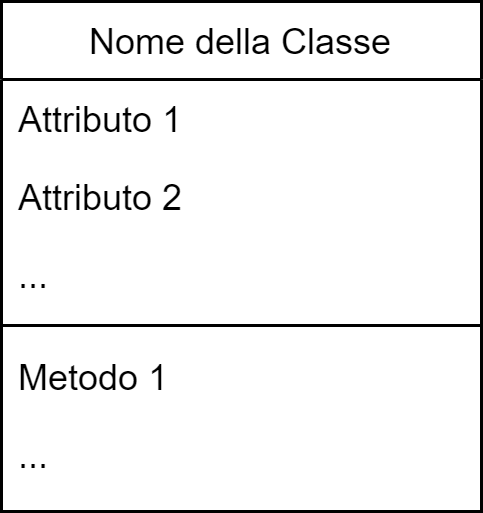
\includegraphics[width=0.25\textwidth]{classe.png}
        \caption{Rappresentazione di una classe.}
        \end{figure}

        Di seguito vengono elencate tutte le possibili relazioni:
        \begin{itemize}
            \item \textbf{Dipendenza}: La relazione di dipendenza tra due classi è rappresentata da una freccia tratteggiata con la punta, che parte dalla classe dipendente A e punta alla classe da cui si origina la dipendenza B. Questa freccia indica che eventuali modifiche nella classe B potrebbero influenzare o avere un impatto sulla classe A;
            \begin{figure}[H]
            \centering
            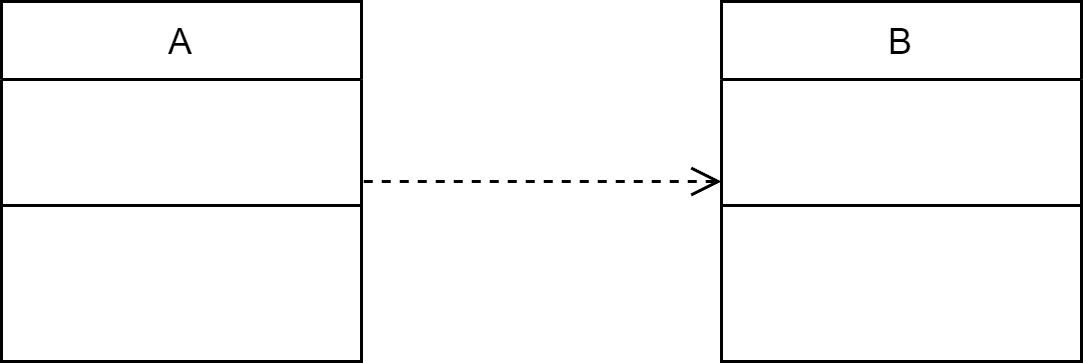
\includegraphics[width=0.5\textwidth]{DipendenzaClasse.png}
            \caption{Rappresentazione della relazione di dipendenza.}
            \end{figure}

            \item \textbf{Aggregazione}: La relazione di aggregazione rappresenta un legame di tipo "part of" tra due classi, in cui una classe è associata ad un'altra ma può esistere anche indipendentemente da essa. Questa relazione viene utilizzata quando una classe A (contenitore) contiene un riferimento ad un oggetto di tipo B (contenuto). L'aggregazione è rappresentata graficamente con una linea che collega le due classi, con un rombo vuoto posto vicino alla classe che rappresenta il contenitore;
            \begin{figure}[H]
            \centering
            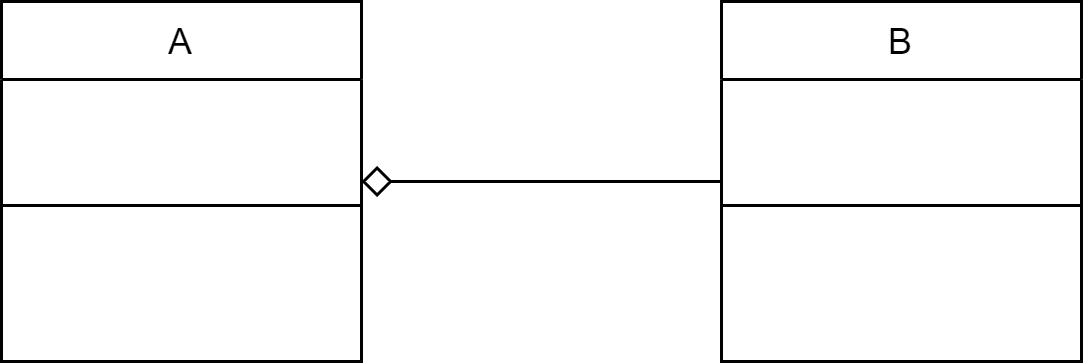
\includegraphics[width=0.5\textwidth]{AggregazioneClasse.png}
            \caption{Rappresentazione della relazione di aggregazione.}
            \end{figure}

            \item \textbf{Composizione}: La relazione di composizione si verifica quando una classe A contiene un oggetto di tipo B e ne ha la responsabilità di crearne e gestirne l'esistenza. La vita di B (contenuto) è vincolata a quella di A (contenitore): se A viene eliminata, anche B viene distrutta. La composizione è rappresentata graficamente con un rombo pieno vicino alla classe che rappresenta il contenitore e una linea che collega le due classi;
            \begin{figure}[H]
            \centering
            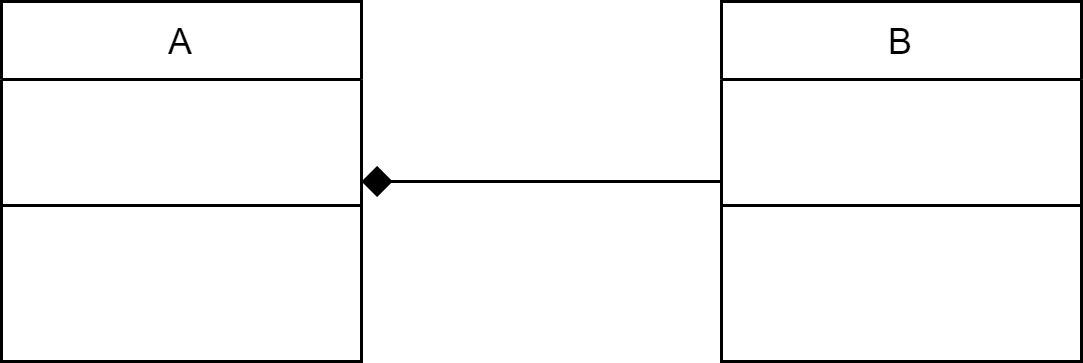
\includegraphics[width=0.5\textwidth]{ComposizioneClasse.png}
            \caption{Rappresentazione della relazione di composizione.}
            \end{figure}

            \item \textbf{Associazione}: La relazione di associazione si verifica quando una classe può contenere riferimenti o istanze di un'altra classe senza implicare una stretta dipendenza. L'associazione è rappresentata graficamente con una linea che collega le classi, spesso accompagnata da valori di molteplicità. Per indicare il senso della relazione, può essere utilizzata una freccia posizionata su uno dei due estremi;
            \begin{figure}[H]
            \centering
            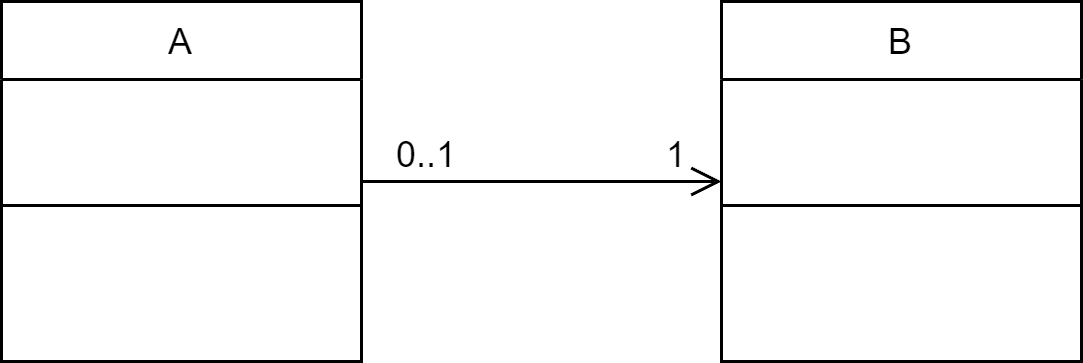
\includegraphics[width=0.5\textwidth]{AssociazioneClasse.png}
            \caption{Rappresentazione della relazione di associazione.}
            \end{figure}

            \item \textbf{Generalizzazione}: La relazione di generalizzazione si verifica quando una classe eredita attributi, comportamenti e relazioni dalla classe genitore. Nello specifico ogni istanza della classe figlia è anche un'istanza della classe genitore, ma con caratteristiche o dettagli aggiuntivi specifici. La generalizzazione è rappresentata graficamente con una freccia vuota che collega la classe figlia (B) alla classe genitore (A).
            \begin{figure}[H]
            \centering
            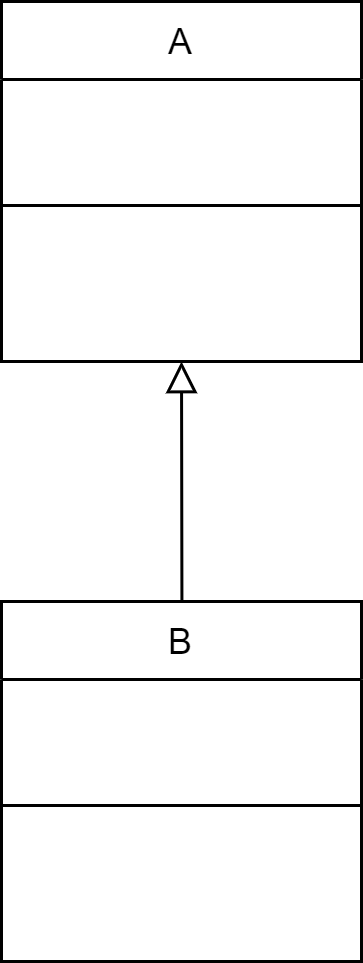
\includegraphics[width=0.15\textwidth]{GeneralizzazioneClasse.png}
            \caption{Rappresentazione della relazione di generalizzazione.}
            \end{figure}
        \end{itemize}

        \paragraph{Metriche}
        \begin{table}[H]
          \centering
          \begin{tabular}{|c|c|}
            \hline
            \textbf{Metrica} & \textbf{Descrizione} \\
            \hline
            MPD09 & Tempo medio di risposta\\
            \hline
            MPD10 & Facilità di utilizzo\\
            \hline
            MPD11 & Tempo medio di apprendimento\\
            \hline
            MPD18 & Versioni browser supportati\\
            \hline
          \end{tabular}
          \caption{Metriche relative all'attività di progettazione}
        \end{table}

    \subsubsection{Codifica}
    \label{codifica}
        \paragraph{Descrizione e Scopo}
        L'attività di codifica rappresenta la fase cruciale in cui le funzionalità richieste dal proponente$_G$ vengono tradotte in istruzioni eseguibili. I Programmatori, incaricati di questa attività, hanno il compito di implementare il design concettuale definito dai Progettisti, seguendo scrupolosamente le linee guida e le norme$_G$ stabilite. Questo metodo di lavoro garantisce che il codice segua accuratamente le specifiche, promuovendo qualità, manutenibilità e coerenza nell'intero progetto$_G$.\\
        L'obiettivo principale della codifica è quindi creare un prodotto software che soddisfi le esigenze del proponente$_G$ e rispetti gli accordi contrattuali. Le aspettative del codice sviluppato includono:
        \begin{itemize}
            \item \textbf{Conformità alle specifiche}: Garantire che il codice traduca fedelmente i requisiti e le funzionalità richieste;
            \item \textbf{Chiarezza e leggibilità}: Scrivere codice autoesplicativo, riducendo la necessità di commenti superflui;
            \item \textbf{Ottimizzazione delle prestazioni}: Assicurare che il codice sia efficiente e scalabile;
            \item \textbf{Testabilità}: Integrare test$_G$ di unità e di integrazione per verificare la correttezza e l'affidabilità.
        \end{itemize}

        \paragraph{Norme di codifica}
        Per garantire uno sviluppo del codice coerente e di alta qualità, i Programmatori adottano le seguenti regole:
        \begin{itemize}
            \item \textbf{Nomi significativi}: Utilizzare nomi univoci, oltre che chiari e descrittivi per variabili, metodi e classi, evitando abbreviazioni ambigue;
            \item \textbf{Indentazione}: Applicare uno schema di formattazione uniforme per migliorare la leggibilità del codice. Ogni livello di annidamento deve essere chiaramente separato con un tab o spazi coerenti;
            \item \textbf{Lunghezza dei metodi}: I metodi devono essere brevi e focalizzati su una singola responsabilità, per favorire test$_G$ di unità efficaci.
        \end{itemize}

        \paragraph{Strumenti utilizzati}
        Il team di sviluppo utilizza strumenti che supportano la scrittura di codice leggibile, mantenibile e conforme agli standard. Tra questi:
        \begin{itemize}
            \item \textbf{Visual Studio Code}: L'IDE principale scelto per la codifica, grazie alla sua versatilità e facilità d'uso.
        \end{itemize}

        \paragraph{Integrazione}
        Durante la fase di integrazione le diverse componenti, moduli o servizi del progetto$_G$ vengono combinati e testati per creare un sistema$_G$ coeso e funzionante.\\
        L'obiettivo principale dell'integrazione è garantire che tutte le parti del sistema$_G$ interagiscano correttamente e rispettino i requisiti funzionali e di prestazione definiti.
        Sin dalle prime fasi di sviluppo è necessario integrare le componenti del prodotto adottando un approccio solido ma flessibile, essenziale per garantire che le soluzioni esplorate durante la fase di Proof of Concept (PoC) siano utili una volta che il progetto$_G$ entra nella fase di sviluppo del Minimum Viable Product (MVP).\\
        Questa fase è supportata da test$_G$ di integrazione che verificano che i moduli lavorino correttamente insieme. L'integrazione continua, supportata da strumenti automatizzati come CI$_G$/CD (Continuous Integration/Continuous Delivery), permette di garantire che ogni nuova modifica non comprometta l'affidabilità del sistema$_G$, mantenendo un flusso di lavoro agile$_G$ e risolvendo eventuali problemi o incompatibilità prima che si presentino nel sistema$_G$ finale.\\

        \paragraph{Verifica}
        La verifica è una fase cruciale del ciclo-di-vita$_G$ del software, durante la quale si controlla che il codice sviluppato rispetti le specifiche e soddisfi i requisiti stabiliti. Questo processo$_G$ garantisce che il prodotto sia conforme agli standard di qualità, riducendo al minimo la presenza di errori e assicurando un'implementazione efficiente e mantenibile.\\
        Il processo$_G$ di verifica comprende sia un'analisi statica del codice, per rilevare eventuali errori o problemi di formattazione, sia l'esecuzione di test$_G$ mirati per validare le funzionalità implementate.\\

        \paragraph{Metriche}
        \begin{table}[H]
          \centering
          \begin{tabular}{|c|c|}
            \hline
            \textbf{Metrica} & \textbf{Descrizione} \\
            \hline
            MPD05 & Code coverage\\
            \hline
            MPD06 & Statement coverage\\
            \hline
            MPD07 & Branch$_G$ coverage\\
            \hline
            MPD08 & Condition coverage\\
            \hline
            MPD12 & Coefficiente di accoppiamento fra classi\\
            \hline
            MPD13 & Linee di codice per metodo\\
            \hline
            MPD14 & Parametri per metodo\\
            \hline
            MPD15 & Attributi per classe\\
            \hline
            MPD16 & Structure Fan IN\\
            \hline
            MPD17 & Structure Fan OUT\\
            \hline
          \end{tabular}
          \caption{Metriche relative all'attività di codifica}
        \end{table}

\newpage
\section{Processi di supporto}
    \subsection{Documentazione}

    \subsubsection{Descrizione e Scopo}
    La documentazione$_G$ è l'insieme delle informazioni che accompagna lo sviluppo di un prodotto software, svolge un ruolo essenziale nella descrizione del prodotto per coloro che lo realizzano, lo distribuiscono e lo utilizzano.\\
    Il suo scopo principale è quello di semplificare il lavoro dei membri del team durante l'intero ciclo-di-vita$_G$ del progetto$_G$, monitorando tutti i processi e le attività coinvolte. Questo permette di migliorare il risultato finale e semplifica notevolmente la manutenzione.

    \subsubsection{Lista documenti}
    I documenti prodotti nel contesto della realizzazione del progetto$_G$ sono:
    \begin{itemize}
        \item [-] \textit{Analisi\_dei\_Requisiti}
        \item [-] \textit{Glossario}
        \item [-] \textit{Norme\_di\_Progetto}
        \item [-] \textit{Piano\_di\_Progetto}
        \item [-] \textit{Piano\_di\_Qualifica}
        \item [-] \textit{Verbali esterni}
        \item [-] \textit{Verbali interni}
    \end{itemize}

    \subsubsection{Ciclo di vita documenti e Versionamento$_G$}
    I documenti seguono due workflow distinti a seconda che si tratti di verbali (interni o esterni) oppure di documenti più corposi, e le versioni delle modifiche successive apportate ai documenti seguono il sistema$_G$ di versionamento$_G$ indicato di seguito.\\

        \paragraph{Versionamento dei documenti}
        Il sistema$_G$ adottato dal team per il versionamento$_G$ dei documenti è il sistema$_G$ di versionamento$_G$ semantico: \{x.y.z\}, in cui ogni numero ha un significato specifico:\\
        \begin{itemize}
            \item "x" indica la versione maggiore, incrementata per cambiamenti incompatibili con versioni precedenti;
            \item "y" rappresenta la versione minore, usata per aggiungere informazioni compatibili;
            \item "z" è la versione di patch, aggiornata per correzioni di errori poco significativi e retrocompatibili.
        \end{itemize}
        Questo sistema$_G$ aiuta il team a comprendere velocemente l'impatto di un aggiornamento fatto ad un documento prodotto.\\

        \paragraph{Workflow verbali}
        I verbali seguono il seguente workflow:
        \begin{enumerate}
            \item Creazione del documento a partire da un template diverso a seconda che si tratti di un verbale interno o esterno (la versione iniziale del documento corrisponde a \{0.1.0\});
            \item Compilazione dei campi della sezione Registro modifiche;
            \item Redazione del documento indicando la durata dell'incontro, i partecipanti (interni ed esterni) e la piattaforma utilizzata. Seguono la sintesi di quanto fatto e una descrizione di ciascuna delle considerazioni fatte e successive decisioni prese;
            \item Nella sezione Decisioni prese si compila una
            tabella in cui ciascuna azione da intraprendere viene associata ad una issue$_G$ corrispondente;
            \item Creazione di una pull-request (PR) dal branch$_G$ Verbali al branch$_G$ Main;
            \item Verifica del verbale prodotto da parte del Verificatore
            indicato nel Registro modifiche del documento stesso;
            \item Se CI$_G$ sono correzioni o ulteriori modifiche da fare, queste devono essere indicate nella sezione Registro modifiche, e successivamente verificate;
            \item Solo se la verifica dà esito positivo si può passare alla fase di approvazione, anch'essa da verificare;
            Da questo punto se il verbale è interno si passa all'ultimo passaggio mentre se il verbale è esterno va mandato all'azienda Synclab$_G$ perché venga firmato;
            \item Quando il documento è completo l'ultimo Verificatore
            chiude la pull-request ed esegue il merge$_G$ nel branch$_G$ Main.
        \end{enumerate}

        \paragraph{Workflow altri documenti}
        Gli altri documenti seguono il seguente workflow:
        \begin{enumerate}
            \item Creazione di un branch$_G$ dedicato esclusivamente alla redazione di un documento specifico;
            \item Creazione del documento a partire da un template comune a tutti i documenti (esclusi i verbali). La versione iniziale del documento corrisponde a \{0.1.0\};
            \item Creazione di una draft pull-request dal branch$_G$ corrispondente a tale documento al branch$_G$ Main;
            \item Compilazione dei campi della sezione Registro modifiche;
            \item Redazione del documento o di una sua sezione;
            \item Verifica della documentazione$_G$ prodotta da parte del Verificatore indicato nel Registro modifiche e associato alle modifiche effettuate in quella seduta di lavoro;
            \item Se CI$_G$ sono correzioni o ulteriori modifiche da fare, queste devono essere indicate nella sezione Registro modifiche, e successivamente verificate;
            \item Si ripetono le operazioni indicate dal punto \{4\} al punto \{6\} fino a quando il documento non è stato completato;
            \item Quando il documento è completo l'ultimo Verificatore
            chiude la draft pull-request ed esegue il merge$_G$ nel branch$_G$ Main. Successivamente, si procede ad eliminare il branch$_G$ dedicato, solo se non sono previsti ulteriori sviluppi.
        \end{enumerate}

    \subsubsection{Template in \LaTeX}
    Per la stesura dei documenti, viene utilizzato un template in formato \LaTeX. Questo template ha lo scopo di semplificare la redazione dei documenti, garantire la coerenza e risparmiare del tempo, in modo da rendere la produzione dei documenti più efficiente e professionale. Sono stati sviluppati tre diversi modelli di template:
    \begin{itemize}
        \item Documenti ufficiali;
        \item Verbale Interno;
        \item Verbale Esterno.
    \end{itemize}

    \subsubsection{Nomenclatura}
    La nomenclatura dei documenti prevede che il nome del file sia composto dal nome del documento e dalla versione, separati da underscore (\_), come nell'esempio: "\textit{Piano\_di\_Qualifica\_v1.0.0.pdf}".\\
    Nel caso dei verbali, la nomenclatura prevede l'uso del nome "VerbaleInterno" o "VerbaleEsterno", seguito dalla data nel formato "YYYY-MM-DD", con un trattino (-) che li unisce, come nell'esempio "\textit{VerbaleEsterno-2024-11-10.pdf}".\\

    \subsubsection{Struttura documenti}

        \paragraph{Prima Pagina}
        \begin{itemize}
            \item \textbf{Logo Team}: Situato in alto al centro;
            \item \textbf{Titolo}: \begin{itemize}
            \item Nome del documento, qualora non sia un verbale;
            \item Verbale Interno;
            \item Verbale Esterno.
            \end{itemize}
            \item\textbf{Sottotitolo}: Nome del capitolato$_G$;
            \item\textbf{Contatti}: Email del team;
            \item\textbf{Logo Università}: Situato in basso a destra.
        \end{itemize}

        \paragraph{Intestazione}
        Su ogni pagina del documento, eccetto la prima, si trova il logo del gruppo seguito dal titolo del documento e dalla sua versione.\\

        \paragraph{Registro modifiche}
        Il registro delle modifiche è una tabella dettagliata che tiene traccia di ogni modifica avvenuta al documento nel corso del tempo. È utile per tenere traccia dell'evoluzione del documento e per consentire a chiunque stia lavorando sul progetto$_G$ di comprendere quali modifiche sono state apportate e quando.
        L'intestazione comprende:
        \begin{itemize}
            \item \textbf{Versione}: Versione del documento;
            \item \textbf{Data}: Data della modifica apportata;
            \item \textbf{Autore}: Autore della modifica;
            \item \textbf{Verificatore}: Autore della verifica;
            \item \textbf{Descrizione}: Cosa è stato modificato o aggiunto al file.
        \end{itemize}

        \paragraph{Indice}
        Nella pagina successiva al registro delle modifiche è presente l'indice, che permette di facilitare la ricerca e la navigazione all'interno del documento.\\

        \paragraph{Verbali}
        I verbali sono dei documenti di sintesi di un incontro che sia interno al team o esterno con l'azienda, per questo motivo la loro struttura è diversa rispetto agli altri documenti ufficiali.\\
        I verbali hanno lo scopo di tenere traccia di chi ha partecipato agli incontri ed in particolare quali decisioni sono state prese.\\
        Sono composti da 2 sezioni principali:
        \begin{itemize}
            \item \textbf{Durata e partecipanti}: Viene indicata la data di inizio e fine dell'incontro, insieme al luogo in cui si è svolto. Successivamente, vengono elencati i nomi dei partecipanti del gruppo. Se il verbale è esterno, vengono inclusi anche i partecipanti dell'azienda Synclab$_G$;
            \item \textbf{Sintesi e Decisioni/Obiettivi}: La prima sezione contiene un riassunto degli argomenti trattati durante il meeting, mentre la seconda include un elenco delle decisioni prese, collegate alle issue$_G$ corrispondenti tramite una tabella.
        \end{itemize}
        Inoltre, per i verbali esterni è presente una sezione per la convalida del documento mediante una firma.\\

    \subsubsection{Convenzioni stilistiche}
        \paragraph{Stile del testo}
        \begin{itemize}
            \item \textbf{Grassetto}: Viene utilizzato per i titoli di sezioni/sottosezioni/paragrafi di un documento e per le definizioni di termini negli elenchi puntati;
            \item \textbf{Corsivo}: Viene utilizzato per i nomi dei documenti;
            \item \textbf{Link}: Sono collegamenti ipertestuali, consentono di accedere a risorse esterne o interne, come altre pagine, sezioni, immagini o file, con un semplice click;
            \item \textbf{Glossario}: I termini che si possono ritrovare nel \textit{Glossario} sono seguiti dall'apice $_G$.
        \end{itemize}

        \paragraph{Formato delle date}
        \'E stato adottato il formato "YYYY-MM-DD", ovvero:
        \begin{itemize}
            \item \textbf{YYYY}: anno con 4 cifre;
            \item \textbf{MM}: mese con 2 cifre;
            \item \textbf{DD}: giorno con 2 cifre.
        \end{itemize}

    \subsubsection{Strumenti}
    Il gruppo ha deciso di utilizzare i seguenti strumenti:
    \begin{itemize}
        \item \textbf{Git}: Strumento per il controllo di versione distribuito impiegato dal gruppo per gestire i documenti e le versioni successive di essi prodotte in maniera asincrona dai membri;
        \item \textbf{GitHub}: Piattaforma di versionamento$_G$ e repository$_G$ per la documentazione$_G$. Permette la gestione del codice sorgente, il controllo delle modifiche tramite funzionalità come le issue$_G$ e le pull-request (PR), facilitando la collaborazione all’interno di un team di sviluppo;
        \item \textbf{\LaTeX}: Linguaggio scelto per la redazione dei documenti, spesso utilizzato in ambito accademico, scientifico e tecnico;
        \item \textbf{Overleaf}: Servizio utilizzato dal gruppo per la creazione e modifica sincrona da parte di due o più componenti di file .tex usati per produrre documentazione$_G$.
    \end{itemize}

    \subsection{Gestione della configurazione}
    \label{gestione-configurazione}
    \subsubsection{Descrizione e Scopo}
    Il processo$_G$ di gestione della configurazione identifica le norme$_G$ che sono state adottate durante lo svolgimento del progetto$_G$ al fine di garantire la tracciabilità, la coerenza e la comprensibilità del codice e della documentazione$_G$ prodotta dal gruppo.\\
    Il suo scopo è gestire e organizzare le modifiche al codice o alla documentazione$_G$, garantendo che siano accompagnate dalle motivazioni alla base dei cambiamenti effettuati e dai relativi autori.

    \subsubsection{Project Board}
    Per la gestione delle attività viene utilizzata la board di Github$_G$, che offre una struttura organizzativa chiara ed efficiente. All'interno della board sono presenti diverse corsie di stato, ognuna delle quali descrive il progresso delle attività e sono suddivise come segue:
    \begin{enumerate}
        \item \textbf{ToDo}: attività identificate e pianificate ma ancora da avviare;
        \item \textbf{In Progress}: attività in corso, assegnate ad uno o più membri del gruppo;
        \item \textbf{Done}: attività completate, in attesa di verifica.
    \end{enumerate}

    \subsubsection{Repository}
    Il gruppo utilizza due repository$_G$ all'interno della propria organizzazione Github$_G$:
    \begin{itemize}
        \item \href{https://github.com/SevenBitsSwe/7BitsDocs}{https://github.com/SevenBitsSwe/7BitsDocs}: questa repository$_G$ è utilizzata per revisionare e mantenere aggiornati i documenti redatti, permettendo ai membri del gruppo di gestire in modo efficiente la documentazione$_G$;
        \item \href{https://github.com/SevenBitsSwe/PoC}{https://github.com/SevenBitsSwe/PoC}: questa repository$_G$ è dedicata alla condivisione e verifica del codice sorgente relativo al prodotto software realizzato per la revisione RTB$_G$. Viene utilizzata dal team per lavorare sul codice del prodotto, consentendo una gestione centralizzata dello sviluppo e delle modifiche apportate al software.
    \end{itemize}

        \paragraph{Struttura della repository$_G$ 7BitsDocs}
        Per ogni documento è stato creato un branch$_G$ dedicato, al fine di lavorare in modo efficace ed efficiente, evitando di generare conflitti e prevenendo il caricamento sulla pagina web di documenti non ancora approvati, ossia con una versione precedente alla 1.0.0. Per questo motivo, è stato adottato un modello git-flow semplificato, che prevede l'uso di più branch$_G$ di lavoro separati. Di conseguenza, nessuno dei branch$_G$ dedicati deve essere eliminato.\\
        Ogni branch$_G$, derivante direttamente dal branch$_G$ principale Main, contiene diverse cartelle relative alle fasi del progetto$_G$: una per la Candidatura e una per la RTB$_G$, ciascuna contenente i documenti redatti per quella specifica fase. Inoltre, sono presenti una cartella per le immagini utilizzate nei documenti, due cartelle per la gestione della pagina web e i file di supporto (README, templates, ecc.).

        \paragraph{Struttura della repository$_G$ PoC$_G$}
        Per quanto riguarda il prodotto software sviluppato per la revisione RTB$_G$, sono stati creati diversi branch$_G$, ognuno derivante direttamente dal branch$_G$ Main, e ciascuno utilizzato per esplorare e approfondire una specifica tecnologia. Solo una volta presa la decisione di implementare una determinata tecnologia, viene effettuato un merge$_G$ in un branch$_G$ specifico che include l'intero prodotto. Solo quest'ultimo può successivamente confluire nel branch$_G$ Main attraverso una pull-request, a condizione che ogni modifica sia stata verificata e approvata.
    
    \subsubsection{Pagina web} 
    La pagina web, accessibile al link \href{https://sevenbitsswe.github.io/7BitsDocs/}{https://sevenbitsswe.github.io/7BitsDocs/}, è stata progettata per offrire un'esperienza chiara e intuitiva, organizzando la documentazione$_G$ in base alle diverse fasi per cui è stata redatta. Grazie all'integrazione di una Github$_G$ Action, la pagina si aggiorna automaticamente ad ogni modifica apportata nel branch$_G$ Main del repository$_G$ 7BitsDocs, garantendo che siano visibili soltanto i documenti approvati.

    \subsubsection{Controllo dei termini del glossario}
    È stato sviluppato uno script in Python$_G$ per verificare la presenza dei termini definiti nel \textit{Glossario} all'interno dei vari documenti. Lo script utilizza espressioni regolari per identificare i termini nei documenti e confrontarli con quelli inclusi nella lista predefinita, formattandoli secondo lo standard del \textit{Glossario}. Quando rileva un termine della lista non correttamente formattato, lo script aggiunge automaticamente una $_G$ a pedice per garantirne la conformità.\\
    Tutti i termini inclusi nel \textit{Glossario} devono essere formattati correttamente ogni volta che compaiono nel documento, e non solo alla loro prima occorrenza. Questa regola semplifica la consultazione e favorisce una migliore comprensione dei termini chiave all'interno della documentazione$_G$.

    \subsection{Verifica}
    \label{verifica}
    \subsubsection{Descrizione e Scopo} 
    La verifica è un processo$_G$ essenziale che deve essere applicato a tutti gli altri processi per poterli considerare completati. Il suo scopo principale è quello di assicurare che i prodotti siano corretti e che aderiscano ai vincoli individuati ed elencati nel documento \textit{Piano\_di\_Qualifica}. Le attività di verifica sono assegnate ai verificatori, che si impegnano a far rispettare i vincoli di qualità presenti nel \textit{Piano\_di\_Qualifica}, correggendo e/o segnalando qualora siano presenti contenuti non conformi agli standard.
    \subsubsection{Strumenti}
    Gli strumenti utilizzati per agevolare il processo$_G$ di verifica sono i seguenti:
    \paragraph{GitHub}
    Github$_G$ fornisce un servizio di code review integrato nel meccanismo delle pull-request, consentendo ai verificatori di visualizzare le ultime modifiche. Dopo aver completato la verifica del documento, il Verificatore può aggiungere commenti con correzioni o suggerimenti di miglioramento e richiedere delle modifiche. In alternativa, può approvarla e passare alla verifica di altri prodotti in attesa di revisione nel repository$_G$.\\
    Il sistema$_G$ di review di Github$_G$ permette all'intero team di tracciare le modifiche apportate nel repository$_G$. Inoltre, è possibile assegnare regole alle pull-request per garantire che la verifica venga effettuata da almeno due verificatori prima di eseguire il merge$_G$ nel branch$_G$ Main.

    \subsubsection{Analisi statica}
    L'analisi statica è un tipo di verifica che viene effettuata sul prodotto software o sulla documentazione$_G$ senza dover eseguire il sistema$_G$ software. Serve ad accertare la conformità con le regole adottate, verificare l'assenza di difetti e la presenza di proprietà desiderate, garantendo un livello ottimale di qualità. Le due principali tecniche sono Inspection$_G$ e Walkthrough$_G$. Il gruppo preferisce l'approccio ad Inspection$_G$, così da ridurre il tempo di verifica affinché l'autore possa dedicarsi alla stesura di altri documenti o codice.
    
    \paragraph{Inspection}
    Il Verificatore segue una sequenza di passaggi prestabiliti per verificare che si stiano rispettando le regole presenti nel \textit{Piano\_di\_Qualifica}.
    
    \paragraph{Walkthrough}
    Il Verificatore e l'autore del prodotto da verificare discutono sulle modifiche da apportare. Questo processo$_G$ richiede la presenza sincrona e la collaborazione di entrambi i ruoli, dunque risulta più complessa dell'Inspection in termini organizzativi. Viene effettuato un controllo ad ampio spettro dell'oggetto, senza avere un'idea precisa di cosa andare a verificare.

    \subsubsection{Analisi dinamica}
    L'analisi dinamica viene condotta direttamente sul prodotto software attraverso la sua esecuzione effettiva. Questo tipo di analisi si suddivide in diverse tipologie di test$_G$, ciascuna finalizzata a verificare aspetti specifici del funzionamento software. Ogni test$_G$ corrisponde all'esecuzione di un programma, e simula il comportamento di singole parti di codice su un insieme finito di casi di prova.\\
    Questa procedura misura la qualità del prodotto e assicura che esso raggiunga correttamente il suo scopo. I test$_G$ effettuati devono essere ripetibili nel tempo per assicurare un funzionamento persistente durante tutto lo svolgimento del prodotto software.
    
    \subsubsection{Classificazione dei test$_G$}
    Tutti i test$_G$ che verranno eseguiti sono presenti nel documento \textit{Piano\_di\_Qualifica} ed il Verificatore è tenuto a svolgerli, riportandone gli esiti all'interno dello stesso documento.\\
    Ad ogni test$_G$ devono essere attribuiti:
    \begin{itemize}
    \item \textbf{Stato iniziale}: parametri del software al momento dell'esecuzione del test$_G$;
    \item \textbf{Input}: dati forniti in entrata per l'esecuzione del test$_G$;
    \item \textbf{Output}: risultati attesi in uscita, dato uno specifico input.
    \end{itemize}
    Inoltre i test$_G$ sono divisi in varie categorie:

    \paragraph{Test di unità}
    Test$_G$ eseguiti su singole unità del software, come funzioni o metodi, in modo indipendente dal resto del sistema$_G$. L'obiettivo è assicurare che ogni unità di codice funzioni correttamente.\\
    Devono essere eseguiti per primi visto che le unità garantiscono il corretto funzionamento dei singoli metodi che poi verranno integrati tra di loro.\\
    Sono presenti due tipi di test$_G$ di unità:
    \begin{itemize}
    \item \textbf{Funzionale}: verificano che ogni unità esegua le funzioni specificate nel design, facendo riferimento solo alla specifica input-output dell'oggetto di verifica;
    \item \textbf{Strutturale}: verificano la logica interna dell'oggetto di verifica esaminando il codice sorgente dell'unità.
    \end{itemize}

    \paragraph{Test di integrazione}
    Test$_G$ eseguiti per controllare la corretta interazione tra le varie unità del software. Questo tipo di test$_G$ vengono eseguiti dopo la conferma che tutti i test$_G$ di unità siano passati con successo.\\
    Vi sono due tipi di integrazione:
    \begin{itemize}
      \item \textbf{Bottom-up}: l'integrazione parte dalle componenti di sistema$_G$ con minori dipendenze e un maggiore valore interno. Richiede pochi mock ma ritarda la messa a disposizione di funzionalità visibili all'utente;
      \item \textbf{Top-down}: l'integrazione parte dalle componenti di sistema$_G$ con maggiori dipendenze e un maggiore valore esterno. Richiede molti mock ma integra prima le funzionalità visibili all'utente.
    \end{itemize}

    \paragraph{Test di sistema$_G$}
    Test$_G$ eseguiti per controllare che i requisiti specificati durante l'analisi-dei-requisiti siano rispettati, garantendo che tutte le componenti siano integrate correttamente.\\
    L'obiettivo di questi test$_G$ è di accertarsi che l'intero sistema$_G$ lavori come entità unica, verificando che tutte le singole componenti funzionino insieme. Vengono eseguiti al completamento dei test$_G$ di integrazione.

    \paragraph{Test di regressione}
    Garantiscono che le modifiche apportate al codice non introducano nuovi difetti o danneggino il sistema$_G$ precedentemente funzionante.\\
    Consistono nella ripetizione selettiva delle tipologie dei test$_G$ elencati precedentemente e devono essere eseguiti ogni volta che si effettuano modifiche al codice.

    \paragraph{Test di accettazione}
    Sono gli ultimi test$_G$ da passare prima del rilascio del software. Servono a garantire che il prodotto finale soddisfi le aspettative del proponente$_G$ e degli utenti finali.

    \paragraph{Classificazione dei test$_G$}
    I test$_G$ vengono identificati in base alla loro tipologia e tramite un codice numerico, specifico all'interno della categoria. I test$_G$ devono avere la seguente forma:
    \begin{quote}
    \textbf{T[Tipologia Test$_G$][Codice]}\\
    \end{quote}
    Dove:
    \item [-] \textbf{Tipologia}:
    \begin{itemize}
        \item [*] \textbf{U}: Unità;
        \item [*] \textbf{I}: Integrazione;
        \item [*] \textbf{S}: Sistema$_G$;
        \item [*] \textbf{A}: Accettazione.
    \end{itemize}

    \paragraph{Stato dei test$_G$}
    Nel \textit{Piano\_di\_Qualifica} ogni test$_G$ viene seguito dal suo stato:
    \begin{itemize}
    \item \textbf{NI}: Il test$_G$ non è stato implementato;
    \item \textbf{NP}: il test$_G$ non è stato passato, con esito negativo;
    \item \textbf{P}: il test$_G$ è stato passato, con esito positivo.
    \end{itemize}

\subsection{Gestione della Qualità}

    \subsubsection{Descrizione e Scopo}
     La qualità viene assicurata tramite processi di verifica e validazione, che permettono di monitorare l'aderenza agli standard definiti. Una volta stabiliti i criteri qualitativi nel \textit{Piano\_di\_Qualifica}, il gruppo si impegna a seguire le best-practices per ogni fase del progetto$_G$, dai processi di sviluppo alla produzione degli artefatti. La responsabilità di garantire l'applicazione degli standard è delegata ai Verificatori, che certificano la conformità dei prodotti e dei processi agli obiettivi qualitativi.\\
     Il processo$_G$ di gestione della qualità ha come obiettivo primario garantire che il software e i processi del ciclo-di-vita$_G$ del progetto$_G$ rispettino i requisiti specificati e siano allineati ai piani stabiliti. Attraverso l'adozione di standard qualitativi ben definiti, si mira a creare un prodotto affidabile ed efficiente, conforme alle aspettative e agli obiettivi concordati con il proponente$_G$.
    
    \subsubsection{Aspettative}
    CI$_G$ si attende che:
    \begin{itemize}
        \item Il gruppo rispetti gli standard qualitativi definiti di comune accordo;
        \item La documentazione$_G$ prodotta sia chiara, coerente e conforme agli obiettivi del progetto$_G$;
        \item I prodotti software sviluppati soddisfino i requisiti funzionali e non funzionali concordati;
        \item Le pratiche di verifica e validazione siano eseguite regolarmente e con accuratezza.
    \end{itemize}
    
    \subsubsection{Metriche e Strumenti}
    Per monitorare e valutare la qualità, vengono utilizzate specifiche metriche, adattate ai diversi processi coinvolti. Queste metriche forniscono uno strumento oggettivo per analizzare il lavoro svolto e identificare eventuali criticità. Le metriche sono descritte nel dettaglio nel \textit{Piano\_di\_Qualifica} e includono:
    \begin{itemize}
        \item \textbf{Metriche di processo$_G$}: utilizzate per valutare l'efficienza e l'efficacia dei processi produttivi e organizzativi;
        \item \textbf{Metriche di prodotto}: impiegate per analizzare la qualità degli artefatti e dei prodotti finali.
    \end{itemize}
    
    \subsubsection{Struttura e identificazione delle metriche}
    Le metriche adottate nel progetto$_G$ sono identificate e descritte secondo una struttura standardizzata che ne facilita il riconoscimento e l'utilizzo. Ogni metrica è caratterizzata dai seguenti elementi:
    \begin{itemize}
        \item \textbf{Codice}: identificativo univoco della metrica, definito nel formato:
    \begin{quote}
        \textbf{M[abbreviazione][numero]}
    \end{quote}
    Dove:
    \begin{itemize}
        \item \textbf{[abbreviazione]}: PC se si tratta di qualità di processo$_G$, PD se si tratta di qualità di prodotto.
        \item \textbf{[numero]}: numero progressivo univoco per ciascuna metrica;
    \end{itemize}
    
    \item \textbf{Nome}: il nome completo della metrica;
    \item \textbf{Descrizione}: breve descrizione della funzionalità e dell'ambito di applicazione della metrica.
\end{itemize}

Eventualmente, le metriche possono includere:
\begin{itemize}
    \item \textbf{Formula}: modalità di calcolo della metrica.
\end{itemize}
    
    \subsubsection{Documentazione della Qualità}
    La gestione della qualità è documentata nel \textit{Piano\_di\_Qualifica}, che definisce le metriche e le soglie accettabili per i vari processi e prodotti. Eventuali modifiche agli standard o agli strumenti vengono tracciate e aggiornate in modo continuo per garantire un processo$_G$ di miglioramento costante.

\newpage
\section{Processi organizzativi}
    \subsection{Gestione dei processi}

    \subsubsection{Descrizione e Scopo}
    Come stabilito dallo standard ISO/IEC 12207:1997, il processo$_G$ di gestione comprende tutte le attività necessarie per completare un progetto$_G$ software, in modo tale da garantire il raggiungimento degli obiettivi prefissati nel rispetto dei requisiti, dei tempi e dei costi. Per conseguire questo obiettivo, questo processo$_G$ si compone di una pianificazione dettagliata, un monitoraggio continuo dei progressi e l'adozione tempestiva di azioni correttive, quando necessario.

    \subsubsection{Attività}
    Il processo$_G$ di gestione, come stabilito dallo standard ISO/IEC 12207:1997, si compone delle seguenti attività:
    \begin{enumerate}
        \item \textbf{Pianificazione}: Composta dall'identificazione degli obiettivi da raggiungere, dalla stima delle risorse necessarie, dalla definizione dei ruoli coinvolti e dalle scadenze da rispettare;
        \item \textbf{Monitoraggio e controllo}: Composto dalla verifica continua dello stato di avanzamento rispetto alla pianificazione, con un'analisi degli eventuali scostamenti su tempi, costi e risorse. Se necessario, vengono attuate azioni correttive per riallineare il progetto$_G$ agli obiettivi;
        \item \textbf{Gestione dei rischi}: Composta dall'identificazione dei potenziali rischi, dalla valutazione del loro impatto e della probabilità di occorrenza, e dallo sviluppo ed implementazione di piani di attenuazione per ridurre al minimo gli effetti negativi che potrebbero derivarne;
        \item \textbf{Gestione delle comunicazioni}: Composta dalla gestione delle comunicazioni per garantire un flusso costante di informazioni tra tutte le parti interessate, sia interne al gruppo che esterne come l'azienda proponente$_G$, assicurando che le comunicazioni siano chiare e tempestive;
        \item \textbf{Gestione delle modifiche}: Composta dal riconoscimento e dall'approvazione delle richieste di modifica, dalla valutazione del loro impatto sui tempi e sui costi, e dall'aggiornamento della pianificazione per integrare le modifiche approvate;
        \item \textbf{Revisione e chiusura}: Composta dalla valutazione complessiva del progetto$_G$ al termine delle attività, dall'identificazione delle nozioni apprese e dalla formalizzazione della chiusura del progetto$_G$ con la consegna dei risultati finali.
    \end{enumerate}

    \subsubsection{Pianificazione degli sprint$_G$}
    Include la durata di ogni sprint$_G$ e una lista degli obiettivi da raggiungere entro la sua conclusione. Se si verificano dei rischi, viene aggiunta una sezione che descrive come il gruppo li ha gestiti e l'impatto che hanno avuto sulle attività pianificate. Inoltre, la pianificazione contiene una tabella con i ruoli assegnati ai membri del gruppo e due sezioni separate: una per il preventivo, che indica le ore e i costi stimati per lo sprint$_G$, e una per il consuntivo, che riporta le ore e i costi effettivi per lo stesso periodo.

    \subsubsection{Ruoli di progetto$_G$}
    Durante l'intero sviluppo del progetto$_G$, ciascun membro del gruppo assume sei ruoli distinti, ciascuno con responsabilità ben definite che riguardano specifiche attività di specifici processi.
    Ogni ruolo contribuisce al raggiungimento degli obiettivi del progetto$_G$, risultando essenziale per completare tutte le attività necessarie alla creazione di un prodotto finale di qualità.\\
    I ruoli assunti a rotazione da ciascun membro del gruppo sono i seguenti:

        \paragraph{Responsabile}
        Figura incaricata di supervisionare e coordinare le attività del gruppo, assicurandosi il raggiungimento degli obiettivi del progetto$_G$ nei tempi e nei modi previsti. Si occupa di garantire una comunicazione efficace tra il gruppo e la proponente$_G$, pianifica e gestisce le risorse e valuta eventuali scelte e rischi che ne derivano.\\
        I suoi compiti sono:
        \begin{itemize}
            \item Comunicare con la proponente$_G$ attraverso i canali concordati;
            \item Stesura e avanzamento del documento \textit{Piano\_di\_Progetto};
            \item Redazione dei verbali interni ed esterni;
            \item Creazione e assegnazione delle issue$_G$ ai membri del team;
            \item Creazione dei diari di bordo.
        \end{itemize}

        \paragraph{Amministratore}
        Figura responsabile della creazione, manutenzione e ottimizzazione degli strumenti, delle risorse e dei processi necessari per il corretto svolgimento del progetto$_G$. Supervisiona la configurazione degli ambienti di lavoro e il monitoraggio delle scadenze amministrative, fornendo supporto al gruppo nello svolgimento delle attività.\\
        I suoi compiti sono:
        \begin{itemize}
            \item Configurazione e gestione gli ambienti di lavoro;
            \item Controllare e mantenere gli strumenti necessari per la collaborazione e la comunicazione del gruppo;
            \item Gestione del versionamento$_G$ dei documenti;
            \item Stesura e avanzamento del documento \textit{Norme\_di\_Progetto}.
        \end{itemize}

        \paragraph{Analista}
        Figura responsabile di raccogliere, analizzare e documentare i requisiti del progetto$_G$, traducendoli in casi d'uso. Collabora con la proponente$_G$ per comprendere tutte le specifiche e verifica che il prodotto finale risponda alle esigenze e alle aspettative richieste.\\
        I suoi compiti sono:
        \begin{itemize}
            \item Studiare il dominio del problema e relativo contesto applicativo;
            \item Studiare i bisogni dei committenti;
            \item Stesura del documento \textit{Analisi\_dei\_Requisiti};
            \item Stesura e avanzamento del documento \textit{Piano\_di\_Qualifica};
            \item Studiare i requisiti definendo la loro complessità.
        \end{itemize}

        \paragraph{Progettista}
        Figura specializzata nella progettazione architetturale e strutturale di sistemi software. Si occupa di tradurre i requisiti identificati dagli Analisti in un'architettura dettagliata, inoltre determina le scelte realizzative del progetto$_G$ e supervisiona lo sviluppo, senza occuparsi direttamente della manutenzione.\\
        I suoi compiti sono:
        \begin{itemize}
            \item Determinare le tecnologie, i linguaggi e i framework$_G$ da utilizzare;
            \item Progettare l'architettura del sistema$_G$, definendo componenti, moduli e interazioni;
            \item Gestire eventuali rischi che possono sorgere durante lo sviluppo;
            \item Supervisionare lo sviluppo per garantire la conformità all'architettura.
        \end{itemize}

        \paragraph{Programmatore}
        Figura incaricata di trasformare l'architettura proposta dai Progettisti in un sistema$_G$ software funzionante. Si occupa dello sviluppo delle componenti principali e di supporto, seguendo specifiche tecniche e garantendo l'aderenza agli standard di qualità e alle linee guida del progetto$_G$.\\
        I suoi compiti sono:
        \begin{itemize}
            \item Tradurre le specifiche tecniche in codice funzionante;
            \item Creazione di test$_G$ per la verifica e validazione del software;
            \item Scrittura di codice chiaro, leggibile e manutenibile;
            \item Risoluzione di eventuali bug$_G$.
        \end{itemize}

        \paragraph{Verificatore}
        Figura che si occupa di controllare che il lavoro svolto dagli altri membri del gruppo sia corretto, assicurandosi che vengano rispettate tutte le norme$_G$ stabilite per il progetto$_G$.\\
        I suoi compiti sono:
        \begin{itemize}
            \item Revisionare e valutare la documentazione$_G$ prodotta dai membri del gruppo;
            \item Analizzare il codice per individuare errori, discrepanze o possibili miglioramenti;
            \item Identificare e segnalare eventuali problemi.
        \end{itemize}

    \subsubsection{Cambio dei ruoli}
    Per garantire che, al completamento del progetto$_G$, ogni membro abbia ricoperto tutti i ruoli indicati, il gruppo si impegna a riassegnare i ruoli ad ogni componente del gruppo all'inizio di ogni sprint$_G$.

    \subsubsection{Tracciamento delle ore}
    Per tracciare il tempo impiegato nei diversi ruoli durante il progetto$_G$, viene utilizzato uno spreadsheet dedicato, disponibile su Google Drive. Al termine di ogni sprint$_G$, viene utilizzato per generare il consuntivo dello sprint$_G$ appena concluso e il preventivo di quello appena iniziato, infine il membro con il ruolo di Responsabile ha il compito di inserire questi elementi all'interno del documento \textit{Piano\_di\_Progetto}.

        \paragraph{Preventivo}
        Il preventivo delle ore è presentato sotto forma di tabella, che dettaglia le ore stimate per ogni membro del gruppo, suddivise per ruolo e riferite al singolo sprint$_G$. Inoltre, è incluso un diagramma circolare che mostra la ripartizione delle ore stimate per ciascun ruolo, offrendo una visione chiara e immediata delle risorse che si pensa di allocare per quello specifico sprint$_G$.

        \paragraph{Consuntivo}
        Il consuntivo delle ore è presentato sotto forma di tabella, che dettaglia le ore effettive registrate per ogni membro del gruppo, suddivise per ruolo e riferite al singolo sprint$_G$. Inoltre, è incluso un diagramma circolare che mostra la ripartizione delle ore effettive per ciascun ruolo, fornendo una visione chiara e immediata delle risorse effettivamente allocate durante lo sprint$_G$.

    \subsubsection{Ticketing}
    Il gruppo utilizza il sistema$_G$ di Issue$_G$ Tracking (ITS) integrato di Github$_G$ per la gestione delle attività. Questo strumento offre una gestione semplice e chiara dei compiti da svolgere, grazie alla possibilità di creare e chiudere le issue$_G$ in modo rapido ed efficiente. Lo stato di avanzamento delle attività è visualizzabile attraverso la project board integrata di Github$_G$, che garantisce una panoramica chiara e aggiornata del progresso del lavoro.\\
    Le issue$_G$ sono composte da:
    \begin{itemize}
        \item \textbf{Titolo}: identifica in modo univoco il compito da svolgere;
        \item \textbf{Descrizione}: fornisce informazioni dettagliate e utili per il completamento del compito;
        \item \textbf{Assegnatario}: specifica il membro del gruppo incaricato di svolgere il compito;
        \item \textbf{Etichetta}: classifica la tipologia del compito, agevolando l'organizzazione delle issue$_G$;
        \item \textbf{Board}: indica a quale project board appartiene la issue$_G$ e permette di specificare ulteriori campi, tra cui:
        \begin{itemize}
            \item \textbf{Stato}: rappresenta l'avanzamento del compito (Todo, In Progress, Done);
            \item \textbf{Priorità}: assegna un livello di urgenza o importanza alla issue$_G$ (Urgente, Importante, Moderato, Secondario);
            \item \textbf{Grandezza}: stima la complessità o il livello di sforzo richiesto per completare il compito (XS, S, M, L, XL);
            \item \textbf{Iterazione}: specifica a quale sprint$_G$ la issue$_G$ è assegnata.
        \end{itemize}
        \item \textbf{Milestone}: identifica il traguardo o obiettivo specifico a cui la issue$_G$ è associata.
    \end{itemize}
    Ogni volta che è necessario completare un compito, si segue la procedura descritta di seguito:
    \begin{enumerate}
        \item Il Responsabile crea la issue$_G$ su Github$_G$, definendone i dettagli principali;
        \item La issue$_G$ viene assegnata ad un membro del gruppo, che si occuperà del compito;
        \item La issue$_G$ viene associata all'iterazione dello sprint$_G$ attuale;
        \item Il membro incaricato sposta la issue$_G$ nello stato “In Progress” quando inizia a lavorarci;
        \item Al completamento del compito, il Verificatore designato viene informato per procedere al controllo;
        \item Il Verificatore esamina il lavoro svolto e comunica l'esito della verifica tramite Github$_G$;
        \item Se la verifica ha esito positivo, la issue$_G$ viene chiusa e spostata nello stato "Done".
    \end{enumerate}

    \subsubsection{Rischi}
    La gestione dei rischi è un processo$_G$ volto a identificare, valutare e affrontare le situazioni avverse che potrebbero influire sul successo del progetto$_G$. Questo approccio prevede l'individuazione dei rischi, la valutazione della loro gravità e occorrenza, la definizione di strategie per mitigarli ed, infine, un monitoraggio costante per rilevare la possibile comparsa di nuovi rischi.\\
    I rischi vengono suddivisi in tre diverse categorie:
    \begin{itemize}
        \item [-] Rischi Tecnologici;
        \item [-] Rischi di Organizzazione;
        \item [-] Rischi di Pianificazione.
    \end{itemize}
    Ogni rischio$_G$ viene classificato seguendo il formato:
    \begin{quote}
         \textbf{R[Tipo][Indice] - [Nome]}
    \end{quote}
    dove:
    \begin{itemize}
        \item \textbf{R}: Abbreviazione di "Rischio";
        \item \textbf{Tipo}: Categoria del rischio$_G$ (T per Tecnologico, O per Organizzazione, P per Pianificazione);
        \item \textbf{Indice}: Identifica univocamente ciascun rischio$_G$;
        \item \textbf{Nome}: Nome del rischio$_G$.
    \end{itemize}

    \subsubsection{Coordinamento}
    Questa attività comprende la gestione delle comunicazioni e degli incontri tra tutte le parti coinvolte nel progetto$_G$, ossia i  membri del gruppo, la proponente$_G$ e i committenti.

    \subsubsection{Comunicazioni}
    Le comunicazioni sono fondamentali per mantenere un flusso costante di informazioni tra le parti coinvolte, garantendo efficienza$_G$ e coordinamento nel progetto$_G$, supportando il buon andamento delle attività e il raggiungimento degli obiettivi prefissati.\\
    Le comunicazioni si suddividono in:

        \paragraph{Comunicazioni interne}
        Le comunicazioni interne avverranno attraverso due canali principali: Telegram e Discord. Telegram, un servizio di messaggistica istantanea, sarà utilizzato per le conversazioni rapide e informali, mentre Discord, una piattaforma che supporta chat e videochiamate, sarà impiegato per le riunioni a distanza e le discussioni più complesse.\\
        Le attività quotidiane e le comunicazioni generali si svolgeranno su Telegram, mentre le questioni critiche saranno affrontate durante degli incontri su Discord.

        \paragraph{Comunicazioni esterne}
        Le comunicazioni esterne avverranno tramite scambio di email, utilizzando l'indirizzo sevenbits.swe.unipd@gmail.com. Questo canale sarà utilizzato per organizzare incontri con la proponente$_G$, inviare documenti da visionare o firmare. Inoltre, su Discord è presente una sezione testuale dedicata alle comunicazioni rapide o dubbi con la proponente$_G$.

    \subsubsection{Riunioni}
    Le riunioni sono fondamentali per il progresso del progetto$_G$, poiché offrono l'opportunità di confrontarsi, prendere decisioni e risolvere eventuali problematiche. Servono anche per monitorare lo stato di avanzamento delle attività e garantire il raggiungimento degli obiettivi prefissati.
    Al termine di ogni riunione, viene redatto un verbale per documentare gli argomenti trattati e le decisioni prese, garantendo così la tracciabilità e la condivisione delle informazioni. Dopo ogni incontro, il Responsabile redige il verbale, includendo tutte le informazioni rilevanti discusse, lo fa verificare e infine il Verificatore richiede l'approvazione tramite un'ulteriore verifica da parte di un altro membro. Nel caso dei verbali esterni, è prevista anche la firma della proponente$_G$.\\
    Le riunioni si distinguono in:

        \paragraph{Riunioni interne}
        Le riunioni interne sono pianificate settimanalmente ogni mercoledì alle ore 16:00 o, in alternativa, subito dopo le riunioni esterne. In caso di necessità, possono essere richieste riunioni straordinarie durante la settimana, organizzate tramite un sondaggio sul canale Telegram. Tutte le riunioni si terranno sul canale Discord del gruppo. I membri del gruppo si impegnano a partecipare attivamente, cercando di garantire la loro presenza. In caso di impossibilità a partecipare, ogni membro potrà recuperare la sintesi delle discussioni e le decisioni prese leggendo il verbale della riunione.

        \paragraph{Riunioni esterne}
        Le riunioni esterne coinvolgono i membri del gruppo, la proponente$_G$ e i committenti. Gli incontri con la proponente$_G$ si terranno sulla piattaforma Google Meet, con l'indirizzo comunicato al gruppo dall'azienda. I membri del gruppo si impegnano a partecipare attivamente, cercando di garantire la loro presenza. In caso di impossibilità a partecipare, ogni membro potrà recuperare la sintesi delle discussioni e le decisioni prese leggendo il verbale della riunione.

    \subsection{Miglioramento}
    \label{miglioramento}
    \subsubsection{Descrizione e Scopo}
    Il miglioramento è un processo$_G$ finalizzato a valutare, misurare, controllare e ottimizzare il ciclo-di-vita$_G$ del software. Il suo scopo principale è garantire che il prodotto soddisfi tutte le aspettative, mantenendo al contempo elevati standard di qualità ed efficienza$_G$.
    Adottando un approccio ciclico, è previsto che ogni fase venga periodicamente rivisitata e perfezionata, permettendo così di identificare e implementare modifiche mirate per un miglioramento continuo del prodotto.\\ 

    \subsubsection{Ciclo di miglioramento continuo}
    Il miglioramento si compone di quattro fasi fondamentali. La prima fase riguarda l'identificazione dei processi organizzativi da applicare alle diverse attività di progetto$_G$ durante l'intero ciclo-di-vita$_G$ del software. Questi processi devono essere adeguatamente documentati e supportati da un sistema$_G$ di controllo che ne consenta lo sviluppo, il monitoraggio e il miglioramento nel tempo.\\
    La seconda fase consiste nell'implementazione dei miglioramenti identificati, assicurando che le modifiche vengano integrate nei processi esistenti. È essenziale aggiornare la documentazione$_G$ per riflettere i cambiamenti apportati, mentre i dati storici, tecnici e di valutazione devono essere raccolti e analizzati per garantire un progresso continuo.\\
    La terza fase prevede la valutazione dei processi, basata sugli obiettivi predefiniti, le metriche adottate e l'analisi dei dati raccolti. Inoltre, la pianificazione e l'effettuazione di revisioni periodiche garantiscono la loro continua idoneità ed efficacia$_G$.\\
    Infine, la quarta fase si concentra sulla standardizzazione e il consolidamento dei miglioramenti, assicurando che i processi evolvano costantemente e prevenendo il rischio$_G$ di regressioni. Questo approccio ciclico permette di mantenere un'elevata qualità ed efficienza$_G$ nel tempo.

    \subsection{Formazione}
    \label{formazione}
    \subsubsection{Descrizione e Scopo}
    La formazione assicura che ogni membro del gruppo sviluppi le competenze necessarie per affrontare con consapevolezza tutte le sfide che potrebbero emergere durante lo svolgimento del progetto$_G$.\\
    Il percorso$_G$ di apprendimento si basa su un'analisi dettagliata delle esigenze espresse dalla proponente$_G$, seguita dall'identificazione delle risorse più adeguate per il raggiungimento degli obiettivi stabiliti.\\
    Attraverso questo processo$_G$ si realizza un progressivo arricchimento delle conoscenze del gruppo, supportato dal consolidamento della comprensione degli strumenti e delle tecnologie adottate.\\
    La formazione risulta un pilastro fondamentale per il successo del progetto$_G$, offrendo al contempo un'opportunità di crescita professionale per tutti i partecipanti.

    \subsubsection{Formazione individuale}
    Durante lo svolgimento del progetto$_G$, ogni membro del gruppo è tenuto ad approfondire autonomamente le tecnologie necessarie per lo sviluppo del prodotto. Il processo$_G$ di apprendimento è facilitato dalla condivisione di conoscenze tra i membri, grazie al contributo di coloro che possiedono maggiore esperienza e competenza.\\
    Questo approccio consente al gruppo di raggiungere un livello uniforme di conoscenze, adeguato al conseguimento degli obiettivi, e favorisce lo sviluppo complessivo del progetto$_G$.

\newpage
\section{Standard di progetto$_G$}

    \subsection{Standard ISO/IEC 12207 - 1995}
    \label{standard_12207}
    Lo standard ISO/IEC 12207 intitolato "Information technology – Software life cycle processes" individua delle linee guida internazionali per la suddivisione dei processi del ciclo-di-vita$_G$  di un prodotto software. Questo standard definisce un framework$_G$ per tali processi per tutto il corso del ciclo-di-vita$_G$ di un prodotto software, dall'ideazione fino al ritiro.\\
    Lo standard suddivide i processi in tre categorie principali che seguono la suddivisione effettuata in questo stesso documento:
    \begin{itemize}
        \item Processi primari;
        \item Processi di supporto;
        \item Processi organizzativi.
    \end{itemize}

        \subsubsection{Processi primari}
        Trattasi dei processi che coinvolgono direttamente creazione, uso e supporto del software, ovvero di quei processi che descrivono
        le attività principali del ciclo-di-vita$_G$ del software, dalla concezione dello stesso fino alla sua realizzazione. Appartenenti a questa categoria sono le attività di analisi-dei-requisiti, progettazione, implementazione, realizzazione e esecuzione di test$_G$ e infine manutenzione del software.

        \subsubsection{Processi di supporto}
        Questa categoria comprende tutti i processi finalizzati a garantire che i processi primari siano svolti in maniera corretta, coerente ed efficiente. Esempi concreti di questi processi possono essere documentazione$_G$, gestione della configurazione, gestione della qualità, verifica e validazione.

        \subsubsection{Processi organizzativi}
        Si tratta dell'insieme dei processi che definiscono la gestione e definizione delle politiche adottate dal gruppo nell'ambito dello
        svolgimento del progetto$_G$.

    \subsection{Standard ISO/IEC 9126 - 1991}
    \label{standard_9126}
    Lo standard ISO/IEC 9126 individua una serie di linee guida e normative, sviluppate dall'ISO (Organizzazione internazionale per la normazione) in collaborazione con l'IEC (Commissione Elettrotecnica Internazionale), finalizzate a descrivere un modello univoco e globalmente riconosciuto di qualità del software. Il modello nasce dalla necessità di fornire alle società di software un approccio organizzato che faciliti e migliori la produzione di software e conseguentemente anche la qualità dello stesso.

        \subsubsection{Qualità del prodotto software}
        Lo standard ISO/IEC:9126 definisce 6 caratteristiche centrali che influenzano la qualità di un software:
        \begin{itemize}
            \item Funzionalità;
            \item Affidabilità;
            \item Usabilità;
            \item Efficienza$_G$;
            \item Manutenibilità;
            \item Portabilità.
        \end{itemize}

        \begin{figure}[H]
        \centering
        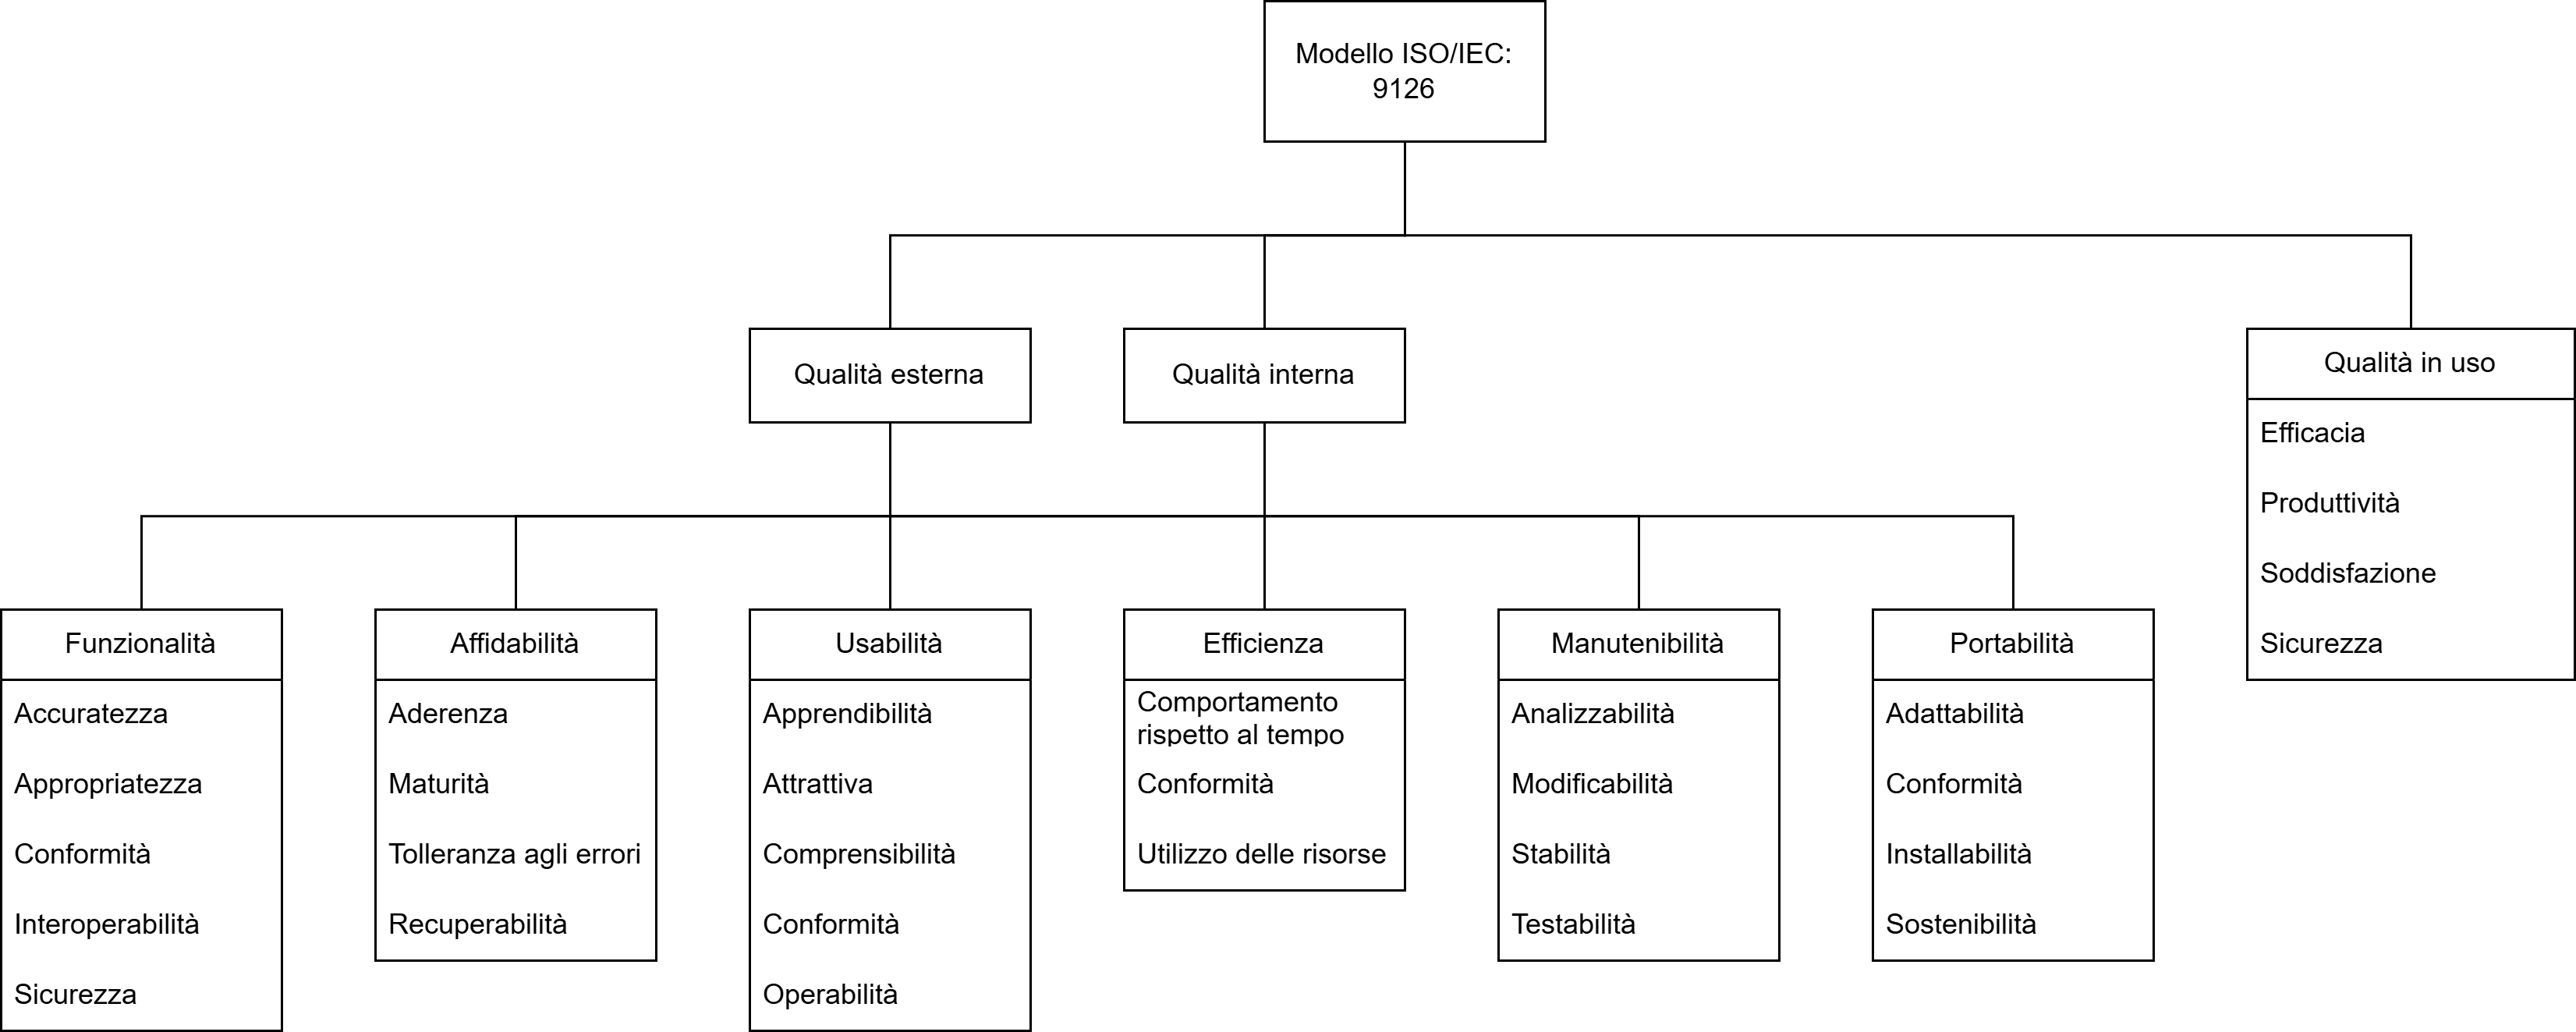
\includegraphics[width=1\textwidth]{Standard9126.png}
        \caption{Schema riassuntivo dello Standard ISO/IEC:9126}
        \end{figure}

            \paragraph{Funzionalità}
            Valuta quanto il software soddisfi i requisiti funzionali espliciti e impliciti. Include cinque sotto-caratteristiche:
            \begin{itemize}
                \item \textbf{Accuratezza}: rappresenta la capacità del software di fornire i risultati concordati;
                \item \textbf{Appropriatezza}: il software deve offrire un appropriato insieme di funzionalità coerenti con il raggiungimento degli obiettivi prefissati all'utente;
                \item \textbf{Conformità}: rappresenta la capacità del prodotto di aderire agli standard e i regolamenti rilevanti nel settore in cui si opera;
                \item \textbf{Interoperabilità}: è la capacità del prodotto software di interagire e cooperare con uno o più sistemi esterni;
                \item \textbf{Sicurezza}: indica la capacità di un prodotto software di proteggere informazioni e dati, garantendo che tutti coloro che interagiscono con tale prodotto (sia persone che altri software) abbiano accesso alle sole informazioni che è loro consentito visualizzare secondo il livello di autorizzazione che possiedono.
            \end{itemize}

            \paragraph{Affidabilità}
            Misura la consistenza con cui il software svolge i suoi compiti mantenendo un certo livello di prestazioni e senza andare incontro a fallimento. Include quattro sotto-caratteristiche:
            \begin{itemize}
                \item \textbf{Aderenza}: misura la frequenza con la quale il software è "up-and-running";
                \item \textbf{Maturità}: un software maturo è stato testato a fondo, pertanto molti bug$_G$ sono stati individuati e risolti;
                \item \textbf{Tolleranza agli errori}: rappresenta la capacità del software di funzionare mantenendo determinati livelli prestazionali anche in presenza di errori;
                \item \textbf{Recuperabilità}: rappresenta la capacità del software di ripristinare un livello adeguato di prestazioni e di recuperare dati rilevanti a seguito di un malfunzionamento.
            \end{itemize}

            \paragraph{Usabilità}
            Misura quanto intuitivo, soddisfacente e facile da usare è un software. Si compone di cinque sotto-caratteristiche:
            \begin{itemize}
                \item \textbf{Apprendibilità}: misura quanto facilmente un nuovo utente può imparare a fare uso di un software;
                \item \textbf{Attrattiva}: misura la capacità del software di essere piacevole da usare per l'utente;
                \item \textbf{Comprensibilità}: rappresenta la facilità con cui gli utenti possono capire le funzionalità offerte da un software;
                \item \textbf{Conformità}: indica la capacità del prodotto di aderire a standard e convenzioni relativi all'usabilità;
                \item \textbf{Operabilità}: indica quanto controllo l'utente ha sul software stesso.
            \end{itemize}

            \paragraph{Efficienza}
            Misura le performance del sistema$_G$ relativamente al quantitativo di risorse usate in determinate condizioni. L'efficienza tiene conto sia della velocità
            del sistema$_G$ software che del suo uso delle risorse fisiche disponibili. Questo aspetto si può ulteriormente dividere in tre sotto-caratteristiche:
            \begin{itemize}
                \item \textbf{Comportamento rispetto al tempo}: è indicatore di quanto velocemente un sistema$_G$ può eseguire un compito o processare una richiesta;
                \item \textbf{Conformità}: rappresenta la capacità del software di aderire a standard e specifiche richieste in termini di efficienza$_G$;
                \item \textbf{Utilizzo delle risorse}: misura quanto efficientemente un software utilizza le risorse fisiche dell'hardware sottostante.
            \end{itemize}

            \paragraph{Manutenibilità}
            Rappresenta la predisposizione di un prodotto software a essere modificato ai fini di migliorarne le performance, renderlo adeguato a un ambiente in evoluzione
            o aggiungere o modificare funzionalità. Un software mantenibile consente di rispondere efficacemente alle necessità degli utenti, a bug$_G$ o problemi rilevati o
            all'evoluzione del panorama tecnologico che circonda il software stesso. Si suddivide in:
            \begin{itemize}
                \item \textbf{Analizzabilità}: rappresenta la facilità con cui è possibile diagnosticare problemi del software;
                \item \textbf{Modificabilità}: indica la facilità con cui è possibile effettuare dei cambiamenti;
                \item \textbf{Stabilità}: rappresenta la robustezza del codice del software nell'evitare effetti inaspettati dovuti a modifiche errate;
                \item \textbf{Testabilità}: rappresenta la facilità con cui è possibile testare il software modificato o prodotto.
            \end{itemize}

            \paragraph{Portabilità}
            Misura la facilità con cui il software si può adattare a un ambiente hardware o software differente da quello originale. La portabilità di un sistema$_G$ si
            traduce nella sua flessibilità o adattabilità. Accorpa le seguenti sotto-categorie:
            \begin{itemize}
                \item \textbf{Adattabilità}: rappresenta la capacità del sistema$_G$ di adattarsi a diversi ambienti operativi senza dover apportare modifiche;
                \item \textbf{Conformità}: è la capacità del prodotto software di aderire a standard e convenzioni relative alla portabilità;
                \item \textbf{Installabilità}: indica la facilità di installazione del software in uno specifico ambiente;
                \item \textbf{Sostituibilità}: rappresenta la capacità del sistema$_G$ di sostituire altri software che svolgono gli stessi compiti nel medesimo ambiente.
            \end{itemize}

\newpage

\section{Metriche per la qualità}
\label{metriche_qualita}
\subsection{Metriche di Qualità del Prodotto}
L'acronimo principale utilizzato in questa sezione è MPD, da Metriche di qualità del Prodotto.

\subsubsection{Funzionalità}
\begin{itemize}
    \item   \textbf{MPD01 - Requisiti Obbligatori Soddisfatti (ROS)}:
            \begin{itemize}
                \item   \textbf{Descrizione}: metrica che valuta quanti dei requisiti obbligatori definiti in fase di analisi-dei-requisiti sono stati soddisfatti.
                \item   \textbf{Formula:}
                        \[
                        ROS = \frac{ROC}{TRO} \cdot 100
                        \]
                        Dove:
                        \begin{itemize}
                            \item $ROC$: requisiti obbligatori coperti.
                            \item $TRO$: requisiti obbligatori totali.
                        \end{itemize}
            \end{itemize}
    \item   \textbf{MPD02 - Requisiti Desiderabili Soddisfatti (RDS)}:
            \begin{itemize}
                \item   \textbf{Descrizione}: metrica che valuta quanti dei requisiti desiderabili definiti in fase di analisi-dei-requisiti sono stati soddisfatti.
                \item   \textbf{Formula:}
                        \[
                        RDS = \frac{RDC}{TRD} \cdot 100
                        \]
                        Dove:
                        \begin{itemize}
                            \item $RDC$: requisiti desiderabili coperti.
                            \item $TRD$: requisiti desiderabili totali.
                        \end{itemize}
            \end{itemize}
    \item   \textbf{MPD03 - Requisiti Opzionali Soddisfatti (RPS)}:
            \begin{itemize}
                \item   \textbf{Descrizione}: metrica che valuta quanti dei requisiti opzionali definiti in fase di analisi-dei-requisiti sono stati soddisfatti.
                \item   \textbf{Formula:}
                        \[
                        RPS = \frac{RPC}{TRP} \cdot 100
                        \]
                        Dove:
                        \begin{itemize}
                            \item $RPC$: requisiti opzionali coperti.
                            \item $TRP$: requisiti opzionali totali.
                        \end{itemize}
            \end{itemize}
    \item   \textbf{MPD04 - Function Point (FP)}:
            \begin{itemize}
                \item   \textbf{Descrizione}: metrica utilizzata per misurare la dimensione funzionale di un prodotto software. Si basa sulle funzionalità offerte dal sistema$_G$ agli utenti finali, e pertanto tiene conto di elementi quali input, output, interfacce, file e query$_G$ interne.
                Il calcolo di tale metrica segue uno schema standardizzato che fa riferimento al IFPUG (International Function Point Users Group), e include cinque componenti principali:
                \begin{enumerate}
                    \item Ingressi esterni (EI).
                    \item Uscite esterne (EO).
                    \item Query$_G$ esterne (EQ).
                    \item File logici interni (ILF).
                    \item File di interfaccia esterni (EIF).
                \end{enumerate}
                Il numero totale di function points viene ponderato sulla base della complessità (alta, media o bassa) relativa a ciascuno di questi elementi.
                \begin{figure}[H]
                \centering
                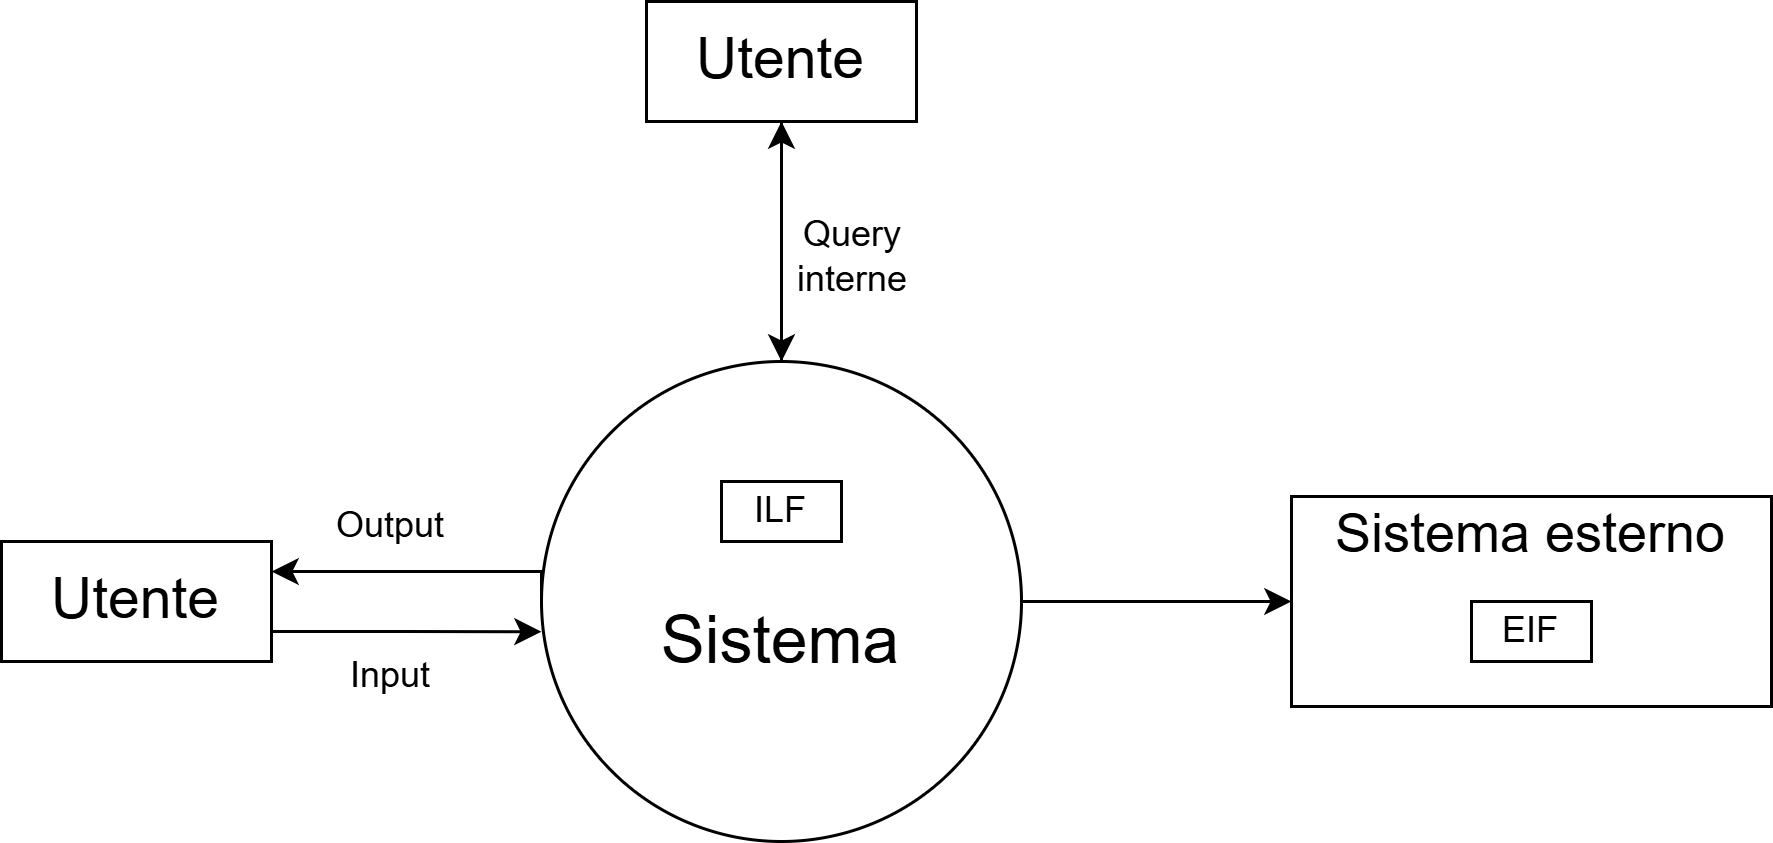
\includegraphics[width=0.7\textwidth]{FunctionPointFigure.png}
                \caption{Schema riassuntivo della metrica Function Point}
                \end{figure}
            \end{itemize}
\end{itemize}

\subsubsection{Affidabilità}
\begin{itemize}
    \item \textbf{MPD05 - Code Coverage}:
    \begin{itemize}
        \item \textbf{Descrizione}: percentuale di codice coperto da test$_G$.
    \end{itemize}
    \item \textbf{MPD06 - Statement Coverage}:
    \begin{itemize}
        \item   \textbf{Descrizione}: percentuale di istruzioni eseguite durante i test$_G$.
        \item   \textbf{Formula:}
                \[
                SC = \frac{IST}{NTIS} \cdot 100
                \]
                Dove:
                \begin{itemize}
                    \item $IST$: istruzioni testate.
                    \item $NTIST$: numero totale istruzioni.
                \end{itemize}
    \end{itemize}

    \item \textbf{MPD07 - Branch$_G$ Coverage}:
    \begin{itemize}
        \item   \textbf{Descrizione}: percentuale di rami decisionali testati.
        \item   \textbf{Formula:}
            \[
            BC = \frac{RDT}{NTR} \cdot 100
            \]
            Dove:
            \begin{itemize}
                \item $RDT$: rami decisionali testati.
                \item $NTR$: numero totale rami decisionali.
            \end{itemize}
    \end{itemize}

    \item \textbf{MPD08 - Condition coverage}:
    \begin{itemize}
        \item   \textbf{Descrizione}: percentuale di condizioni logiche testate.
        \item   \textbf{Formula:}
            \[
            CC = \frac{CLT}{NTCL} \cdot 100
            \]
            Dove:
            \begin{itemize}
                \item $CLT$: condizioni logiche testate.
                \item $NTCL$: numero totale condizioni logiche.
            \end{itemize}
    \end{itemize}

    \item \textbf{MPD09 - Tempo medio di risposta}:
    \begin{itemize}
        \item \textbf{Descrizione}: misura l'efficienza del sistema$_G$ in termini di reattività.
    \end{itemize}
\end{itemize}

\subsubsection{Usabilità}
\begin{itemize}
    \item \textbf{MPD10 - Facilità di utilizzo}:
        \begin{itemize}
            \item \textbf{Descrizione}:  misura la facilità con cui gli utenti possono utilizzare il sistema$_G$.
        \end{itemize}
    \item \textbf{MPD11 - Tempo medio di apprendimento}:
        \begin{itemize}
            \item \textbf{Descrizione}: tempo medio necessario agli utenti per apprendere l'uso del sistema$_G$.
        \end{itemize}
\end{itemize}

\subsubsection{Manutenibilità}
\begin{itemize}
    \item \textbf{MPD12 - Coefficiente di accoppiamento fra classi}:
    \begin{itemize}
        \item \textbf{Descrizione}: misura del numero di classi usate da una singola classe.
    \end{itemize}
    \item \textbf{MPD13 - Linee di codice per metodo}:
      \begin{itemize}
        \item \textbf{Descrizione}: massimo numero di linee di codice consentito per singolo metodo.
      \end{itemize}
    \item \textbf{MPD14 - Parametri per metodo}:
      \begin{itemize}
        \item \textbf{Descrizione}: massimo numero di parametri consentito per singolo metodo.
      \end{itemize}
    \item \textbf{MPD15 - Attributi per classe}:
      \begin{itemize}
        \item \textbf{Descrizione}: massimo numero di attributi consentito per singola classe.
      \end{itemize}
    \item \textbf{MPD16 - Structure Fan IN}:
      \begin{itemize}
        \item \textbf{Descrizione}: rappresenta il numero di moduli, funzioni o classi che chiamano o utilizzano una specifica funzione o modulo, indicando quanto è riutilizzato.
      \end{itemize}
    \item \textbf{MPD17 - Structure Fan OUT}:
      \begin{itemize}
        \item \textbf{Descrizione}: misura il numero di moduli, funzioni o classi che una specifica funzione o modulo utilizza o chiama, evidenziando le sue dipendenze.
      \end{itemize}
\end{itemize}

\subsubsection{Portabilità}
  \begin{itemize}
    \item \textbf{MPD18 - Versioni browser supportati}:
      \begin{itemize}
        \item \textbf{Descrizione}: percentuale delle versioni di browser supportate rispetto al totale delle versioni disponibili.
      \end{itemize}
\end{itemize}

\subsection{Metriche di qualità di Processo$_G$}
L'acronimo principale utilizzato in questa sezione è MPC, da Metriche di qualità del Processo$_G$.

\subsubsection{Processi Primari}
\paragraph{Fornitura}
\begin{itemize}
    \item \textbf{MPC01 - Estimated at Completion (EAC)}:
    \begin{itemize}
        \item   \textbf{Descrizione}: stima il costo totale del progetto$_G$ basandosi sul rendimento attuale.
        \item   \textbf{Formula:}
                \[
                EAC = AC + ETC
                \]
    \end{itemize}
    \item \textbf{MPC02 - Estimate to Complete (ETC)}:
    \begin{itemize}
        \item   \textbf{Descrizione}: stima dei costi rimanenti per completare il progetto$_G$.
        \item   \textbf{Formula:}
                \[
                ETC = BAC - EV
                \]
    \end{itemize}
    \item \textbf{MPC03 - Actual Cost (AC)}:
    \begin{itemize}
        \item \textbf{Descrizione}: indica il costo effettivamente sostenuto per completare il lavoro fino a un certo momento.
    \end{itemize}
    \item \textbf{MPC04 - Earned Value (EV)}:
        \begin{itemize}
            \item \textbf{Descrizione}: misura il valore del lavoro effettivamente realizzato fino a un certo momento del progetto$_G$. Tale metrica è data dalla somma
            dei valori guadagnati fino a quel momento per ciascuna delle attività di cui si compone il progetto$_G$; e ognuno di questi è dato dal budget di tale attività
            moltiplicato per la percentuale di completamento della stessa attività.
        \end{itemize}
    \item \textbf{MPC05 - Planned Value (PV)}:
        \begin{itemize}
            \item \textbf{Descrizione}: rappresenta il valore pianificato del lavoro da completare in un determinato momento.
        \end{itemize}
    \item \textbf{MPC06 - Schedule variance (SV)}:
    \begin{itemize}
        \item   \textbf{Descrizione}: indica se si è in ritardo o in anticipo rispetto al valore pianificato. Un valore negativo indica che si è in ritardo.
        \item   \textbf{Formula:}
            \[
            SV = EV - PV
            \]
    \end{itemize}
    \item \textbf{MPC07 - Cost variance (CV)}:
    \begin{itemize}
        \item   \textbf{Descrizione}: indica se il costo attuale sta superando o meno il budget. Un valore negativo indica che si ha superato il budget.
        \item   \textbf{Formula:}
            \[
            CV = EV - AC
            \]
    \end{itemize}
    \item \textbf{MPC08 - Cost Performance Index (CPI)}:
    \begin{itemize}
        \item   \textbf{Descrizione}: indica quanti obiettivi sono stati raggiunti rispetto al costo sostenuto in determinato periodo di tempo. Un valore negativo indica che il progetto$_G$ è in ritardo rispetto al budget in quanto i costi sostenuti sono superiori al valore del lavoro completato.
        \item   \textbf{Formula:}
            \[
            CPI = \frac{EV}{AC}
            \]
    \end{itemize}
\end{itemize}

\paragraph{Sviluppo}
\begin{itemize}
\item   \textbf{MPC09 - Requisiti Obbligatori Soddisfatti (ROS)}:
            \begin{itemize}
                \item   \textbf{Descrizione}: metrica che valuta quanti dei requisiti obbligatori definiti in fase di analisi-dei-requisiti sono stati soddisfatti.
                \item   \textbf{Formula:}
                        \[
                        ROS = \frac{ROC}{ROT} \cdot 100
                        \]
                        Dove:
                        \begin{itemize}
                            \item $ROC$: requisiti obbligatori coperti.
                            \item $ROT$: requisiti obbligatori totali.
                        \end{itemize}
            \end{itemize}
\item \textbf{MPC10 - Requirements Stability Index(RSI)}:
            \begin{itemize}
                \item   \textbf{Descrizione}: misura la stabilità dei requisiti nel ciclo-di-vita$_G$ di un progetto$_G$. Un RSI$_G$ basso indica che sono stati effettuati molti cambiamenti ai requisiti.
                \item   \textbf{Formula:}
                        \[
                        RSI = 100 - \frac{RA+RC+RR}{RT} \cdot 100
                        \]
                        Dove:
                        \begin{itemize}
                            \item $RA$: requisiti aggiunti dopo l'ultima misurazione.
                            \item $RC$: requisiti modificati dopo l'ultima misurazione.
                            \item $RR$: requisiti rimossi dopo l'ultima misurazione.
                            \item $RT$: requisiti iniziali totali dopo l'ultima misurazione.
                        \end{itemize}
            \end{itemize}
            
\end{itemize}

\subsubsection{Processi di Supporto}
\paragraph{Documentazione}
\begin{itemize}
    \item \textbf{MPC11 - Indice Gulpease}:
    \begin{itemize}
        \item \textbf{Descrizione}: indice di leggibilità di un testo in lingua italiana. Il risultato è in percentuale e cresce al crescere della facilità di comprensione del testo:
            \begin{itemize}
                \item $< 80$: difficile da leggere per persone con la licenza elementare.
                \item $< 60$: difficile da leggere per persone con la licenza media.
                \item $< 40$: difficile da leggere per persone con la licenza superiore.
            \end{itemize}
        \item \textbf{Formula:}
        \[
        IG = 89 + \frac{300 \cdot N_f - 10 \cdot N_l}{N_p}
        \]
        Dove:
        \begin{itemize}
            \item $N_f$: numero totale di frasi nel testo.
            \item $N_l$: numero totale di lettere nel testo.
            \item $N_p$: numero totale di parole nel testo.
        \end{itemize}
    \end{itemize}

    \item \textbf{MPC12 - Correttezza ortografica}:
    \begin{itemize}
        \item \textbf{Descrizione}: metrica che misura il numero di errori ortografici presenti all'interno di un documento.
    \end{itemize}
\end{itemize}

\paragraph{Verifica}
\begin{itemize}
    \item \textbf{MPC13 - Code Coverage}:
    \begin{itemize}
        \item \textbf{Descrizione}: percentuale di codice coperto da test$_G$.
    \end{itemize}
    \item \textbf{MPC14 - Passed test$_G$ cases percentage}:
        \begin{itemize}
            \item \textbf{Descrizione}: percentuale di test$_G$ superati.
        \end{itemize}
\end{itemize}

\paragraph{Gestione della Qualità}
\begin{itemize}
 \item \textbf{MPC15 - Metriche di qualità soddisfatte}:
    \begin{itemize}
        \item \textbf{Descrizione}: percentuale di soddisfacimento delle metriche di qualità stabilite.
    \end{itemize}
\end{itemize}

\subsubsection{Processi Organizzativi}
\paragraph{Gestione dei Processi}
\begin{itemize}
    \item \textbf{MPC16 - Rischi non previsti}:
        \begin{itemize}
            \item \textbf{Descrizione}: numero di rischi non inclusi nelle stime incontrati durante lo svolgimento del progetto$_G$.
        \end{itemize}
    \item \textbf{MPC17 - Efficienza$_G$ Temporale (ET)}:
    \begin{itemize}
        \item   \textbf{Descrizione}: rapporto tra ore produttive ($O_p$) e ore totali ($O_o$) svolte a partire dall'ultima misurazione.
        \item   \textbf{Formula:}
            \[
            ET = \frac{O_p}{O_o}
            \]
    \end{itemize}
\end{itemize}

\end{justify}
\end{document}
